\documentclass[aspectratio=169,10pt]{beamer}
\usetheme{mekatronik}
\renewcommand{\coursetitle}{Mechatronics and Robotics Engineering (50 h)}
\setweek{2}
\setday{5}{Sensors, Measurement \& Integration}
\title[W2D5: Vision, Signals \& Integration]{Sensors, Measurement and System Integration}
\subtitle{6.4 Machine vision \textbullet\ 6.5 Sampling \textbullet\ 6.6 Signal processing \textbullet\ 6.7 Communication \textbullet\ 6.8 Case study \& course wrap-up}
\author{Mechatronics and Robotics Engineering Programme}
\institute{Week 2 \textperiodcentered{} Day 5}
\date{2 weeks \textperiodcentered{} 10 days \textperiodcentered{} 50 hours}

\pgfplotstableset{col sep=space}
\newcommand{\dat}[1]{data/#1.dat}
\tikzset{
  blk/.style={draw=mkBlue,fill=mkPale,thick,rounded corners=1pt,minimum height=7mm,minimum width=12mm,align=center,font=\scriptsize},
  sumn/.style={draw=mkBlue,fill=white,thick,circle,inner sep=0pt,minimum size=4.5mm},
  sig/.style={-{Latex[length=2mm]},thick,mkNavy},
  lbl/.style={font=\scriptsize,text=mkGray},
}
\newcommand{\lbx}[4]{\draw[thick,fill=#4] (#1,0) rectangle (#2,.6); \node[align=center] at ({(#1+#2)/2},.3) {#3};}
\newcommand{\gofurther}[1]{{\footnotesize\color{mkGray}\textbf{\color{mkMid}Going further:} #1}}
% little frame triad (x red-ish orange, y blue)
\newcommand{\triad}[3]{\draw[-{Latex},mkOrange,thick] (#1) -- ++(#2:.6); \draw[-{Latex},mkBlue,thick] (#1) -- ++(#2+90:.6); \node[font=\tiny,mkNavy,anchor=north east] at (#1) {#3};}

\newcommand{\VisionCredit}{Industrial machine-vision camera: Ginkgomaier, CC BY-SA 4.0, via Wikimedia Commons}
\newcommand{\CheckerCredit}{Three-plane chessboard calibration target: Brian moore81, CC BY-SA 4.0, via Wikimedia Commons}
\newcommand{\TagCredit}{}
\newcommand{\StereoCredit}{}
\newcommand{\KukaCredit}{Oleg Yunakov, CC BY-SA 4.0, via Wikimedia Commons}
\begin{document}

\begin{frame}[plain]\titlepage\end{frame}

% =====================================================================
\begin{frame}{Agenda and learning outcomes}
\begin{columns}[T]
\column{.52\textwidth}
\small
\renewcommand{\arraystretch}{1.12}
\begin{tabularx}{\linewidth}{@{}l X r@{}}
\toprule
\textbf{Code} & \textbf{Session} & \textbf{Time}\\
\midrule
6.4 & Machine vision in robotics & 60 min\\
6.5 & Sampling and digitisation & 60 min\\
6.6 & Signal processing and filters & 60 min\\
6.7 & Communication and integration & 60 min\\
6.8 & Integration case study \& course wrap-up & 60 min\\
\bottomrule
\end{tabularx}

\vspace{2mm}
{\footnotesize\color{mkGray} 5 h net teaching time; 10-min breaks roughly every hour are extra.}
\column{.45\textwidth}
\begin{keybox}[By the end of today you can \dots]
\small
\checkitem\ project a 3D point into a camera image\\
\checkitem\ explain calibration and hand--eye setup\\
\checkitem\ apply the Nyquist rule and size an ADC\\
\checkitem\ write a one-line digital low-pass filter\\
\checkitem\ explain how a complementary filter fuses sensors\\
\checkitem\ choose a network for each link in a robot cell\\
\checkitem\ build a latency and error budget for a cell
\end{keybox}
\end{columns}
\end{frame}

% =====================================================================
\begin{frame}{What we learned yesterday (W2D4)}
\begin{columns}[T]
\column{.5\textwidth}
\centering
\begin{tikzpicture}[font=\scriptsize,node distance=2.5mm,
  day/.style={draw=mkBlue,fill=mkPale,thick,rounded corners=2pt,minimum height=7mm,align=left,text width=5.6cm}]
  \node[day] (a) {\textbf{5.6} Conveyors, AGV/AMR, FMS cells, cobots};
  \node[day,below=of a] (b) {\textbf{5.7} Safety: risk assessment, ISO 10218, PL, light curtains};
  \node[day,below=of b] (c) {\textbf{6.1} Accuracy, precision, resolution, range, linearity};
  \node[day,below=of c] (d) {\textbf{6.2} Encoders, resolvers, IMU};
  \node[day,below=of d] (e) {\textbf{6.3} Force/torque, proximity, range, LiDAR};
  \node[day,below=of e,fill=mkCream,draw=mkOrange] (f) {\textbf{Today} From the sensor signal to a working robot cell};
  \draw[sig,mkOrange] (e) -- (f);
\end{tikzpicture}
\column{.47\textwidth}
\begin{defbox}[Three ideas we reuse today]
\small
\checkitem\ \term{Resolution} is the smallest step a sensor can show; \term{accuracy} is how close it is to the truth.\\[1mm]
\checkitem\ An \term{IMU} gives angular rate (gyro) and acceleration --- both imperfect.\\[1mm]
\checkitem\ A \term{homogeneous transform} $T$ moves points between frames (W2D1).
\end{defbox}
\begin{notebox}
\small Today: the robot's \emph{eyes} (vision), how a signal becomes \emph{numbers}, how we \emph{clean} them, and how all devices \emph{talk}.
\end{notebox}
\end{columns}
\end{frame}

% =====================================================================
\section{6.4 Machine vision in robotics}

\begin{frame}{Why robots need eyes}
\begin{columns}[T]
\column{.55\textwidth}
\begin{itemize}\small
\item A taught robot repeats a path blindly: parts must always be in the \hl{same place}.
\item A camera tells the robot \emph{where} the part is, \emph{which} part it is, and whether it is \emph{good}.
\item Typical tasks: \term{locate} (pick from a conveyor or bin), \term{inspect} (defects, presence), \term{read} (barcodes), \term{guide} (seam tracking in welding).
\item \term{2D vision}: one camera, parts on a known plane. \term{3D vision}: stereo, structured light or time-of-flight.
\end{itemize}
\column{.42\textwidth}
\centering
\begin{tikzpicture}[font=\scriptsize]
  % conveyor
  \draw[thick,mkGray,fill=mkLight] (0,0) rectangle (4.6,.35);
  \foreach \x in {.2,4.4}{\draw[mkGray,thick] (\x,.17) circle (.17);}
  \foreach \x/\r in {.8/20,2.0/-35,3.3/60}{\draw[fill=mkOrange!60,draw=mkOrange,rotate around={\r:(\x,.6)}] (\x-.25,.45) rectangle (\x+.25,.75);}
  % camera
  \draw[fill=mkNavy] (1.7,2.4) rectangle (2.3,2.8); \draw[fill=mkNavy] (1.85,2.4) rectangle (2.15,2.25);
  \draw[mkSky,dashed] (1.88,2.25) -- (.6,.4); \draw[mkSky,dashed] (2.12,2.25) -- (3.6,.4);
  \node[above] at (2,2.8) {camera};
  % robot
  \draw[very thick,mkBlue] (4.3,1.0) -- (4.3,1.9) -- (3.6,2.3) -- (3.3,1.2);
  \fill[mkNavy] (4.05,.9) rectangle (4.55,1.05);
  \node[right] at (4.35,1.5) {robot};
  \node[below,mkGray] at (2.3,0) {parts arrive at random angles};
\end{tikzpicture}

\vspace{2mm}
\IfFileExists{../../figures/r25_vision_camera.jpg}{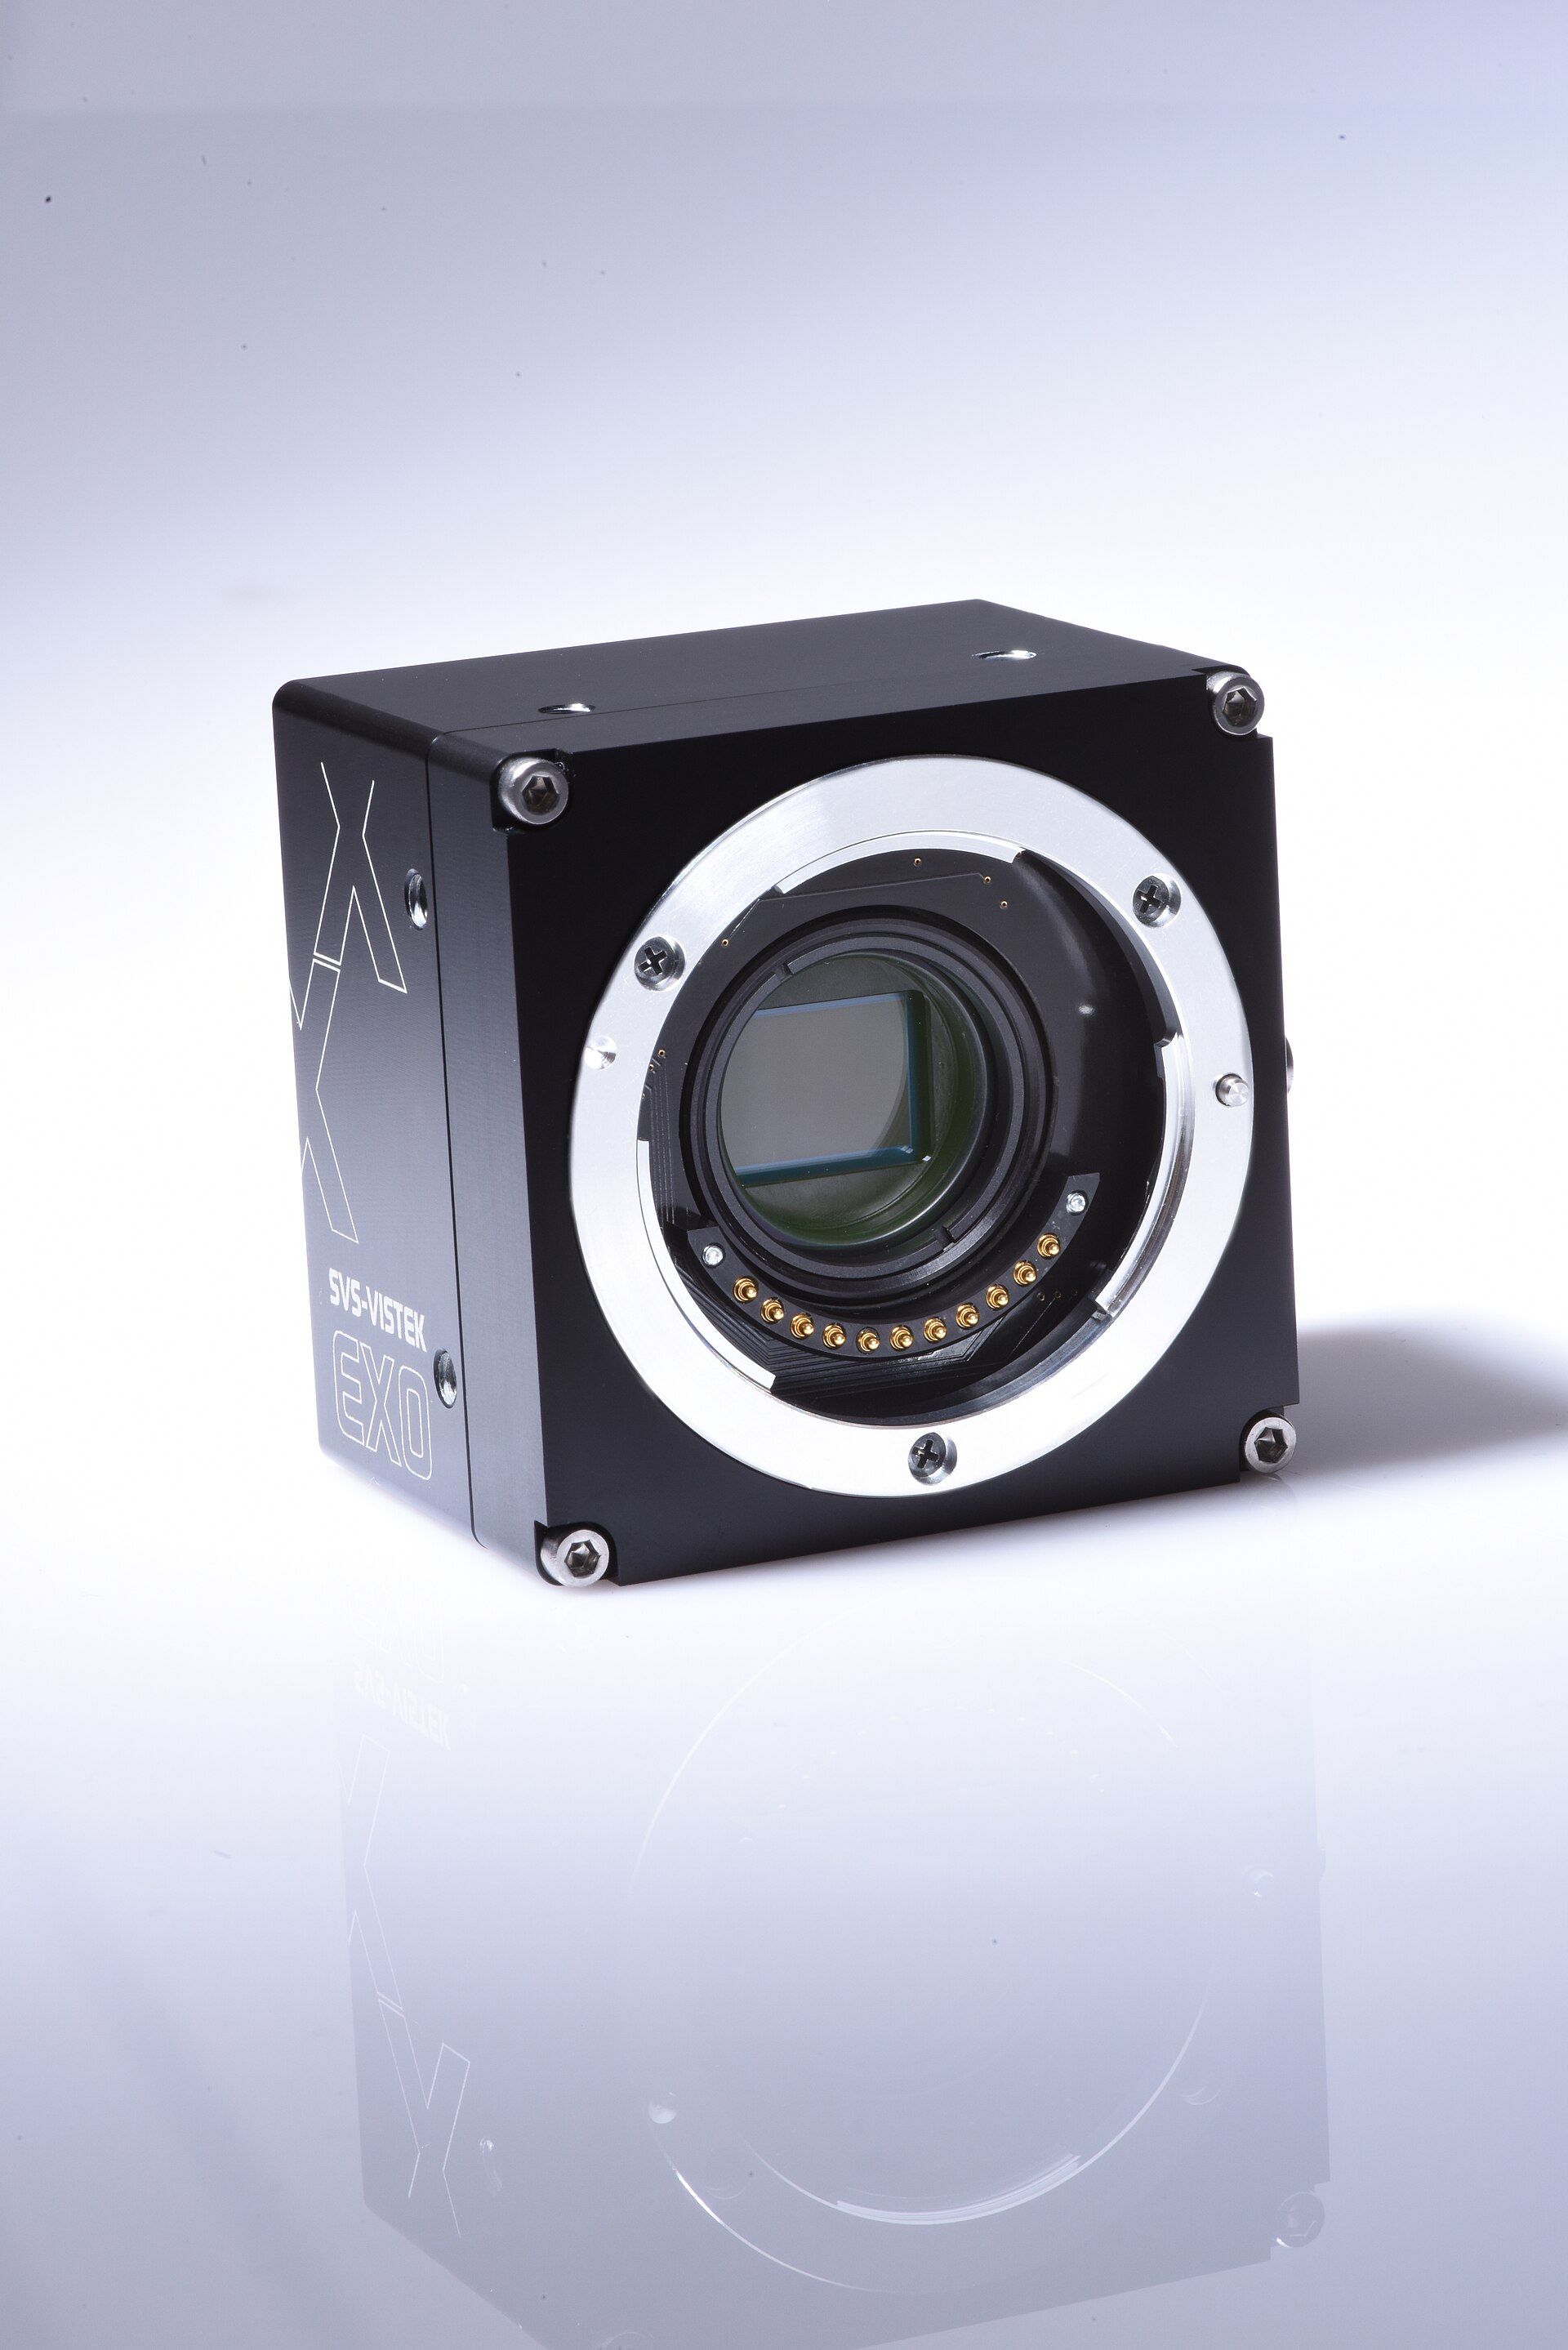
\includegraphics[height=2.0cm]{../../figures/r25_vision_camera.jpg}\\
\credit{\VisionCredit}}{}
\end{columns}
\end{frame}

% ---------------------------------------------------------------------
\begin{frame}{Refresher: the pinhole camera}
\begin{columns}[T]
\column{.52\textwidth}
\centering
\begin{tikzpicture}[font=\scriptsize]
  \draw[mkGray,thin] (-1.6,0) -- (4.6,0) node[right]{optical axis $Z$};
  \draw[very thick,mkNavy] (0,-1.2) -- (0,-.05); \draw[very thick,mkNavy] (0,.05) -- (0,1.2);
  \node[mkNavy,above] at (0,1.2) {pinhole};
  \draw[thick,mkMid] (-1.2,-1.1) -- (-1.2,1.1); \node[mkMid,above] at (-1.2,1.1) {image};
  \draw[mkOrange,very thick,-{Latex}] (4,0) -- (4,1.4) node[right]{$X$};
  \draw[mkOrange,dashed] (4,1.4) -- (-1.2,-.42);
  \draw[mkOrange,very thick,-{Latex}] (-1.2,0) -- (-1.2,-.42) node[left]{$x$};
  \draw[{Latex}-{Latex}] (-1.2,-1.35) -- (0,-1.35) node[midway,below]{$f$};
  \draw[{Latex}-{Latex}] (0,-1.35) -- (4,-1.35) node[midway,below]{$Z$};
\end{tikzpicture}

\begin{itemize}\small
\item Like a dark room with a small hole: the scene appears upside down on the back wall.
\item Similar triangles give the size in the image.
\end{itemize}
\column{.46\textwidth}
\begin{eqbox}
\vspace{-2mm}
\[ u = f_x\,\frac{X}{Z} + c_x,\qquad v = f_y\,\frac{Y}{Z} + c_y \]
\vspace{-4mm}
\end{eqbox}
{\small $X,Y,Z$ [m]: point in the camera frame; $f_x,f_y$ [px]: focal length in pixels; $c_x,c_y$ [px]: image centre; $u,v$ [px]: pixel.}

\begin{keybox}[Worked example]
\small
1.\ $f_x=\SI{1000}{px}$, point at $X=\SI{0.10}{m}$, $Z=\SI{0.50}{m}$\\
2.\ $u-c_x=1000\cdot0.10/0.50=\SI{200}{px}$\\
3.\ One pixel at $Z=\SI{0.5}{m}$ covers $0.5/1000=\SI{0.5}{mm}$\\
4.\ Same object at \SI{1}{m}: half the pixels
\end{keybox}
\end{columns}
\end{frame}

% ---------------------------------------------------------------------
\begin{frame}{The camera model: intrinsics and lens distortion}
\begin{columns}[T]
\column{.5\textwidth}
\begin{eqbox}
\vspace{-2mm}
\[
\begin{bmatrix}u\\v\\1\end{bmatrix} \sim
\underbrace{\begin{bmatrix}f_x&0&c_x\\0&f_y&c_y\\0&0&1\end{bmatrix}}_{K\ \text{(intrinsics)}}
\begin{bmatrix}X/Z\\Y/Z\\1\end{bmatrix}
\]
\vspace{-4mm}
\end{eqbox}
\begin{itemize}\small
\item \term{Intrinsic} parameters: belong to the camera + lens ($f_x,f_y,c_x,c_y$, distortion).
\item \term{Extrinsic} parameters: where the camera is, a transform $T$ like in W2D1.
\item Real lenses bend straight lines: \term{radial distortion}, $r_d=r\,(1+k_1r^2+k_2r^4)$.
\end{itemize}
\column{.47\textwidth}
\centering
\begin{tikzpicture}[font=\scriptsize,scale=.9]
  \begin{scope}
    \foreach \i in {-2,...,2}{\draw[mkSky] (\i*.4,-.8) -- (\i*.4,.8); \draw[mkSky] (-.8,\i*.4) -- (.8,\i*.4);}
    \node[below] at (0,-.9) {ideal};
  \end{scope}
  \begin{scope}[xshift=2.3cm]
    \foreach \i in {-2,...,2}{
      \draw[mkOrange,domain=-1:1,samples=25,smooth,variable=\t] plot ({.8*(\i/2)*(1-0.12*((\i/2)^2+\t^2))},{.8*\t*(1-0.12*((\i/2)^2+\t^2))});
      \draw[mkOrange,domain=-1:1,samples=25,smooth,variable=\t] plot ({.8*\t*(1-0.12*((\i/2)^2+\t^2))},{.8*(\i/2)*(1-0.12*((\i/2)^2+\t^2))});}
    \node[below] at (0,-.9) {barrel};
  \end{scope}
  \begin{scope}[xshift=4.6cm]
    \foreach \i in {-2,...,2}{
      \draw[mkMid,domain=-1:1,samples=25,smooth,variable=\t] plot ({.8*(\i/2)*(1+0.12*((\i/2)^2+\t^2))},{.8*\t*(1+0.12*((\i/2)^2+\t^2))});
      \draw[mkMid,domain=-1:1,samples=25,smooth,variable=\t] plot ({.8*\t*(1+0.12*((\i/2)^2+\t^2))},{.8*(\i/2)*(1+0.12*((\i/2)^2+\t^2))});}
    \node[below] at (0,-1.0) {pincushion};
  \end{scope}
\end{tikzpicture}

\vspace{2mm}
\begin{notebox}
\small The symbol $\sim$ means ``equal up to a scale factor'': all points on one ray through the pinhole land on the same pixel. \hl{One camera cannot see depth.}
\end{notebox}
\end{columns}
\end{frame}

% ---------------------------------------------------------------------
\begin{frame}{Camera calibration: measuring $K$ and the distortion}
\begin{columns}[T]
\column{.5\textwidth}
\begin{enumerate}\small
\item Print a \term{checkerboard} with known square size (e.g.\ \SI{25}{mm}).
\item Take 15--30 images from different angles and distances.
\item Software finds the corners (sub-pixel accurate).
\item It searches $K$, $k_1,k_2$ and each board pose so that projected corners match the found ones.
\item Quality number: \term{reprojection error}, typically $<\SI{0.3}{px}$.
\end{enumerate}
\gofurther{Zhang's method (2000) solves this as a linear estimate followed by non-linear least squares; available in OpenCV and MATLAB.}
\column{.47\textwidth}
\centering
\IfFileExists{../../figures/r25_checkerboard.png}{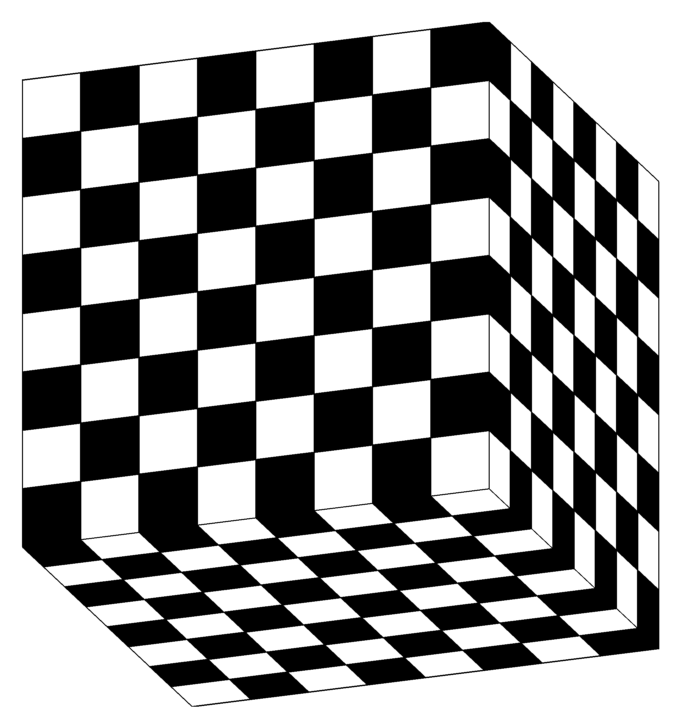
\includegraphics[height=2.5cm]{../../figures/r25_checkerboard.png}\\
\credit{\CheckerCredit}}{%
\begin{tikzpicture}[scale=.35]
  \foreach \i in {0,...,7}{\foreach \j in {0,...,5}{\pgfmathtruncatemacro{\cb}{mod(\i+\j,2)}\ifnum\cb=0 \fill[mkNavy] (\i,\j) rectangle ++(1,1);\fi}}
  \draw[mkNavy] (0,0) rectangle (8,6);
\end{tikzpicture}}

\vspace{2mm}
\begin{keybox}[Analogy]
\small Like tuning a guitar with a reference tone: we show the camera a pattern whose geometry we know exactly and correct the camera until it ``sounds right''.
\end{keybox}
\end{columns}
\end{frame}

% ---------------------------------------------------------------------
\begin{frame}{Pose estimation: where is the object?}
\begin{columns}[T]
\column{.5\textwidth}
\centering
\begin{tikzpicture}[font=\scriptsize]
  % camera
  \draw[fill=mkNavy] (-.3,2.2) rectangle (.3,2.6);
  \coordinate (C) at (0,2.2);
  \node[left] at (-.3,2.4) {camera $\{C\}$};
  % object (square marker) in perspective
  \draw[thick,mkOrange,fill=mkCream] (-1.2,0) -- (1.0,-.3) -- (1.6,.7) -- (-.6,.9) -- cycle;
  \foreach \p in {(-1.2,0),(1.0,-.3),(1.6,.7),(-.6,.9)}{\draw[mkSky,dashed] (C) -- \p; \fill[mkOrange] \p circle (.06);}
  \draw[-{Latex},mkOrange,thick] (.2,.3) -- (1.0,.2) node[right]{$x$};
  \draw[-{Latex},mkBlue,thick] (.2,.3) -- (.5,.8) node[above]{$y$};
  \node[below] at (.2,-.35) {object / marker $\{O\}$};
  \draw[-{Latex},mkMid,thick,bend left=40] (.4,2.2) to node[right,align=left]{$T_{C}^{O}$\\ = rotation\\ + translation} (1.4,.8);
\end{tikzpicture}
\column{.47\textwidth}
\begin{itemize}\small
\item If we know $\ge 4$ points on the object (a CAD model or a printed marker) and see them in the image, we can solve for its \hl{pose} $T_C^O$.
\item This is the \term{Perspective-n-Point} (PnP) problem.
\item \term{Fiducial markers} (ArUco, AprilTag) are black-and-white squares designed to be found and identified quickly.
\end{itemize}
\centering
\begin{tikzpicture}[scale=.22]
  \fill[mkNavy] (0,0) rectangle (8,8); \fill[white] (1,1) rectangle (7,7);
  \foreach \x/\y in {1/1,2/1,4/1,6/1,1/2,3/2,5/2,2/3,3/3,6/3,1/4,4/4,5/4,2/5,3/5,6/5,1/6,4/6,5/6,6/6}{\fill[mkNavy] (\x,\y) rectangle ++(1,1);}
  \node[font=\tiny,mkGray,anchor=west] at (8.4,4) {marker: border + ID code};
\end{tikzpicture}
\end{columns}
\end{frame}

% ---------------------------------------------------------------------
\begin{frame}{Seeing depth: stereo, structured light, time of flight}
\begin{columns}[T]
\column{.5\textwidth}
\centering
\begin{tikzpicture}[font=\scriptsize]
  \fill[mkNavy] (-.25,0) rectangle (.25,.3); \fill[mkNavy] (1.75,0) rectangle (2.25,.3);
  \node[below] at (0,0) {left}; \node[below] at (2,0) {right};
  \draw[{Latex}-{Latex}] (0,-.45) -- (2,-.45) node[midway,below]{baseline $b$};
  \fill[mkOrange] (1.3,1.7) circle (.08) node[right]{point};
  \draw[mkSky] (0,.3) -- (1.3,1.7); \draw[mkSky] (2,.3) -- (1.3,1.7);
  \draw[{Latex}-{Latex},mkGray] (3,.3) -- (3,1.7) node[midway,right]{$Z$};
\end{tikzpicture}

\begin{eqbox}
\vspace{-2mm}
\[ Z=\frac{f\,b}{d} \qquad d=u_L-u_R\ \text{(disparity, px)} \]
\vspace{-4mm}
\end{eqbox}
\begin{keybox}[Worked example]
\small
$f=\SI{700}{px}$, $b=\SI{0.10}{m}$, $d=\SI{35}{px}$ $\Rightarrow$ $Z=700\cdot0.10/35=\SI{2.0}{m}$
\end{keybox}
\column{.47\textwidth}
\begin{tikzpicture}
\begin{axis}[mkplot,width=\linewidth,height=2.8cm,xmin=0.2,xmax=3,ymin=0,ymax=35,
  xlabel={distance $Z$ [m]},ylabel={depth error [mm]}]
\addplot[mkOrange,thick,domain=0.2:3,samples=60]{1000*x^2*0.25/70};
\end{axis}
\end{tikzpicture}
{\scriptsize\color{mkGray} Error $\Delta Z = Z^2\Delta d/(f b)$ for $\Delta d=\SI{0.25}{px}$: grows with $Z^2$.}
\begin{minipage}[t]{.3\linewidth}\vspace{0mm}
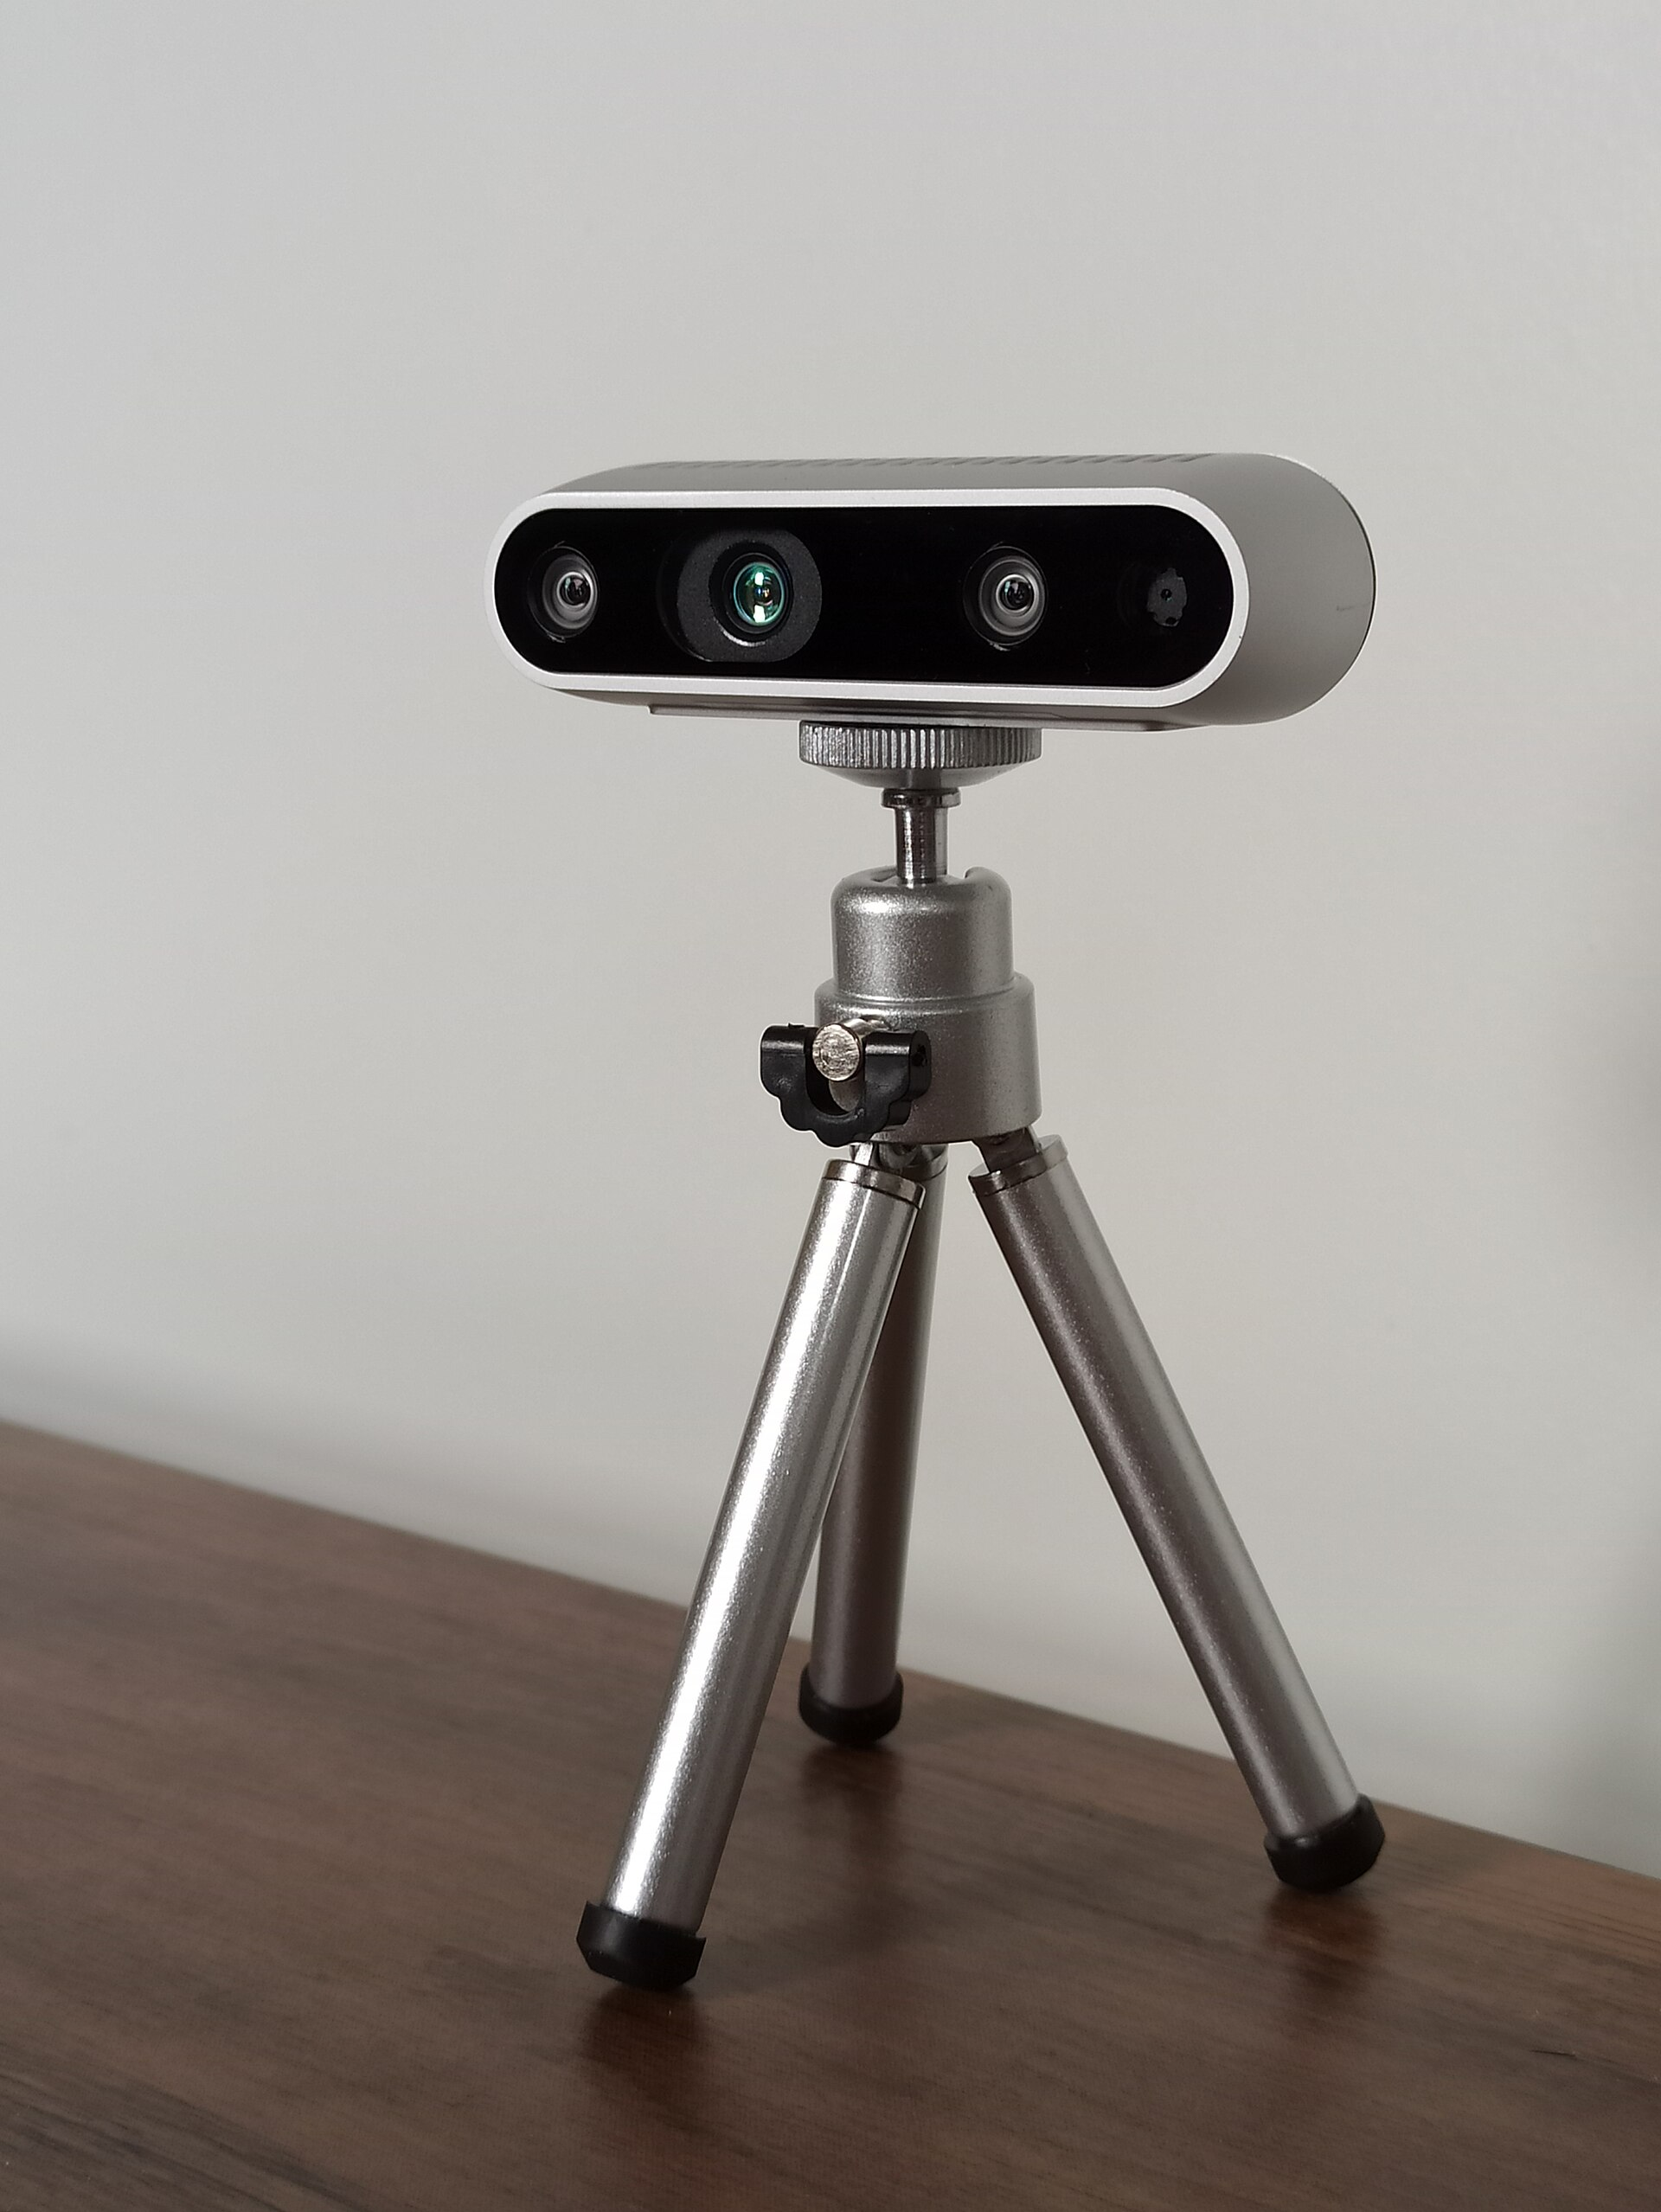
\includegraphics[width=\linewidth,height=1.8cm,keepaspectratio]{../../figures/r25_realsense.jpg}
\end{minipage}\hfill
\begin{minipage}[t]{.6\linewidth}
\begin{itemize}\small
\item \term{Structured light}: project a known pattern, measure how it bends.
\item \term{Time of flight}: measure the light's travel time (like LiDAR).
\end{itemize}
\end{minipage}
\credit{Active stereo depth camera: Marc Auledas, CC BY-SA 4.0, via Wikimedia Commons}
\end{columns}
\end{frame}

% ---------------------------------------------------------------------
\begin{frame}{Hand--eye calibration: where is the camera on the robot?}
\begin{columns}[T]
\column{.55\textwidth}
\centering
\begin{tikzpicture}[font=\scriptsize]
  % eye-in-hand
  \begin{scope}
    \fill[mkNavy] (-.3,0) rectangle (.3,.15);
    \draw[very thick,mkBlue] (0,.15) -- (0,1.3) -- (1.1,1.7) -- (1.5,1.0);
    \fill[mkNavy] (1.62,1.12) rectangle (1.92,1.32);
    \draw[mkSky,dashed] (1.77,1.12) -- (1.4,.0); \draw[mkSky,dashed] (1.77,1.12) -- (2.3,0);
    \fill[mkOrange] (1.85,0) circle (.08);
    \node[below,align=center] at (.9,-.25) {\textbf{eye-in-hand}\\camera on the flange};
  \end{scope}
  % eye-to-hand
  \begin{scope}[xshift=3.6cm]
    \fill[mkNavy] (-.3,0) rectangle (.3,.15);
    \draw[very thick,mkBlue] (0,.15) -- (0,1.3) -- (1.0,1.6) -- (1.4,.8);
    \fill[mkNavy] (1.9,2.2) rectangle (2.3,2.5);
    \draw[mkSky,dashed] (2.1,2.2) -- (1.3,0); \draw[mkSky,dashed] (2.1,2.2) -- (2.8,0);
    \fill[mkOrange] (2.0,0) circle (.08);
    \node[below,align=center] at (1.1,-.25) {\textbf{eye-to-hand}\\camera fixed in the cell};
  \end{scope}
\end{tikzpicture}

\vspace{2mm}
\begin{eqbox}
\vspace{-2mm}
\[ T_B^O = T_B^E\;\textcolor{mkOrange}{T_E^C}\;T_C^O \]
\vspace{-4mm}
\end{eqbox}
{\small base$\rightarrow$flange (robot knows it) $\times$ flange$\rightarrow$camera (\hl{unknown}) $\times$ camera$\rightarrow$object (vision).}
\column{.42\textwidth}
\begin{itemize}\small
\item The camera reports the object in \emph{its own} frame; the robot needs it in the \emph{base} frame.
\item The missing link $T_E^C$ is found by \term{hand--eye calibration}: move the robot to 10--20 poses and look at a fixed checkerboard each time.
\item Eye-to-hand: the unknown is $T_B^C$ instead.
\end{itemize}
\gofurther{this leads to the classic matrix equation $AX=XB$ (Tsai--Lenz 1989, Park--Martin 1994).}
\end{columns}
\end{frame}

% ---------------------------------------------------------------------
\begin{frame}{Worked example: from pixel to robot target}
\begin{columns}[T]
\column{.5\textwidth}
\centering
\begin{tikzpicture}[font=\scriptsize]
  \draw[thick,mkGray,fill=mkLight] (0,0) rectangle (4.6,2.6);
  \node[mkGray,anchor=north west] at (0,2.6) {table seen from above};
  \coordinate (B) at (.3,.3); \triad{B}{0}{base}
  \coordinate (Cc) at (2.5,1.3);
  \draw[-{Latex},mkOrange,thick] (Cc) -- ++(.6,0) node[right]{$x_C$};
  \draw[-{Latex},mkBlue,thick] (Cc) -- ++(0,-.6) node[below]{$y_C$};
  \node[mkNavy,above left] at (Cc) {camera axis};
  \fill[mkRed] (3.0,1.2) circle (.08) node[above right]{part};
  \draw[mkGray,dashed] (B) -- (Cc);
\end{tikzpicture}

\begin{notebox}
\small Fixed camera looks straight down from \SI{0.5}{m}; its axis hits the table at $(600,0)$\,mm in base coordinates; image $y$ points along base $-y$.
\end{notebox}
\column{.48\textwidth}
\begin{keybox}[Step by step]
\small
1.\ Image centre $(c_x,c_y)=(640,480)$; part found at $(u,v)=(840,520)$ px.\\[1mm]
2.\ Offset $(200,\,40)$\,px $\times$ \SI{0.5}{mm/px} $=(100,\,20)$\,mm in the camera frame.\\[1mm]
3.\ Rotate into base: $x_B=+100$, $y_B=-20$\,mm.\\[1mm]
4.\ Add the camera position: target $=(700,\,-20)$\,mm.
\end{keybox}
\begin{itemize}\small
\item Steps 3--4 are just $T_B^C$ applied to a point (W2D1).
\item A \SI{1}{px} error is \SI{0.5}{mm} at the gripper.
\end{itemize}
\end{columns}
\end{frame}

% ---------------------------------------------------------------------
\begin{frame}{Practical vision: light, contrast and speed}
\begin{columns}[T]
\column{.5\textwidth}
\centering
\begin{tikzpicture}[font=\scriptsize]
  \begin{scope}
    \fill[mkNavy] (-.2,2) rectangle (.2,2.3);
    \fill[mkAmber!60] (-1,-.15) rectangle (1,0); \node[below] at (0,-.2) {back light};
    \fill[mkNavy] (-.35,0) rectangle (.35,.35);
    \foreach \x in {-.8,-.5,.5,.8}{\draw[mkAmber,-{Latex}] (\x,0) -- (\x*0.4,1.9);}
    \node[align=center] at (0,-1.0) {sharp silhouette\\(outline, holes)};
  \end{scope}
  \begin{scope}[xshift=3cm]
    \fill[mkNavy] (-.2,2) rectangle (.2,2.3);
    \draw[mkAmber,very thick] (-.6,1.75) -- (-.25,1.75); \draw[mkAmber,very thick] (.25,1.75) -- (.6,1.75);
    \node[right] at (.6,1.75) {ring light};
    \fill[mkMid] (-.4,0) rectangle (.4,.3); \fill[mkGray] (-1,-.15) rectangle (1,0);
    \foreach \x in {-.5,.5}{\draw[mkAmber,-{Latex}] (\x,1.7) -- (\x*.4,.32);}
    \node[align=center] at (0,-1.0) {surface detail\\(print, scratches)};
  \end{scope}
\end{tikzpicture}

\vspace{1mm}
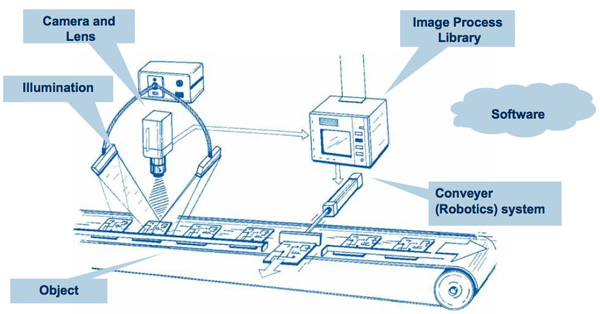
\includegraphics[height=2.1cm]{../../figures/r25_mv_system.jpg}\\
\credit{Machine-vision system: European Editors, CC BY-SA 4.0, via Wikimedia Commons}
\column{.47\textwidth}
\begin{itemize}\small
\item Good \hl{lighting} solves more vision problems than clever software.
\item Moving parts blur: exposure $\SI{1}{ms}$ at \SI{0.5}{m/s} $=\SI{0.5}{mm}$ of smear.
\item Image processing takes time (\SIrange{20}{200}{ms}): the result is \hl{old} when it arrives.
\item Trigger the camera with a signal and \term{time-stamp} the image (more in 6.8).
\end{itemize}
\gofurther{deep-learning detectors handle cluttered bins and varying parts but need training data and a GPU.}
\end{columns}
\end{frame}

% ---------------------------------------------------------------------
\begin{frame}{Check your understanding: machine vision}
\begin{keybox}[Check your understanding]
\large
\begin{enumerate}
\item A camera with $f_x=\SI{800}{px}$ looks at a part \SI{0.4}{m} away. How many millimetres does one pixel cover?
\item Why can a single calibrated camera not tell the height of a part on its own?
\item A stereo camera has an error of \SI{5}{mm} at \SI{1}{m}. Roughly what error do you expect at \SI{2}{m}?
\end{enumerate}
\end{keybox}
\end{frame}

% ---------------------------------------------------------------------
\begin{frame}{Summary and key terms: machine vision}
\begin{columns}[T]
\column{.52\textwidth}
\begin{itemize}\small
\item Pinhole model: $u=f_xX/Z+c_x$; one camera loses depth.
\item Calibration with a checkerboard finds $K$ and lens distortion.
\item Pose estimation (PnP, markers) gives $T_C^O$.
\item Hand--eye calibration links camera and robot: $T_B^O=T_B^E T_E^C T_C^O$.
\item Stereo: $Z=fb/d$, error grows with $Z^2$. Light the scene well.
\end{itemize}
\column{.45\textwidth}
\begin{defbox}[Key terms]
\small
\term{intrinsics} $K$: focal length, image centre\\
\term{extrinsics} camera pose $T$\\
\term{distortion} lens bends straight lines\\
\term{reprojection error} calibration quality [px]\\
\term{PnP} pose from known points\\
\term{disparity} left--right pixel shift
\end{defbox}
{\scriptsize\color{mkGray} [Corke, 2017]; [Szeliski, 2022]; [Zhang, 2000].}
\end{columns}
\end{frame}

\section{6.5 Sampling and digitisation}


% ---------------------------------------------------------------------
\begin{frame}{Refresher: sampling and the wagon-wheel effect}
\begin{columns}[T]
\column{.5\textwidth}
\centering
\begin{tikzpicture}[font=\scriptsize]
  \foreach \i/\rot in {0/0,1/40,2/80}{
    \begin{scope}[xshift=\i*1.9cm]
      \draw[thick,mkNavy] (0,0) circle (.75);
      \foreach \s in {0,45,...,315}{\draw[mkSky] (0,0) -- (\s+\rot:.75);}
      \draw[mkOrange,very thick] (0,0) -- (90+\rot:.75);
      \node at (0,-1.05) {frame \i};
    \end{scope}}
  \draw[-{Latex},mkOrange] (0,1.0) -- (3.8,1.0) node[midway,above]{true: $+40^\circ$ per frame};
  \node[mkRed,align=center] at (1.9,-1.75) {spokes repeat every $45^\circ$: the eye sees\\ $-5^\circ$ per frame $\Rightarrow$ wheel seems to turn \hl{backwards}};
\end{tikzpicture}
\column{.47\textwidth}
\begin{defbox}[Refresher: sampling]
\small
A computer only sees the signal at instants $t=k\,T_s$; the \term{sampling frequency} is $f_s=1/T_s$. Like a film camera taking 24 pictures per second.
\end{defbox}
\begin{eqbox}
\vspace{-2mm}
\[ \text{Nyquist:}\quad f_\text{signal}<\frac{f_s}{2} \]
\vspace{-4mm}
\end{eqbox}
\begin{itemize}\small
\item Faster signals are not lost, they are \hl{disguised} as slower ones: \term{aliasing}.
\item Same as a wagon wheel in a film or a strobe light.
\end{itemize}
\end{columns}
\end{frame}


% ---------------------------------------------------------------------
\begin{frame}{The measurement chain, and a refresher on binary numbers}
\centering
\begin{tikzpicture}[font=\scriptsize,node distance=5mm]
  \node[blk,fill=mkSky!40] (s) {sensor\\(e.g.\ strain gauge)};
  \node[blk,right=of s] (amp) {amplifier\\mV $\rightarrow$ V};
  \node[blk,right=of amp,fill=mkCream,draw=mkOrange] (aaf) {anti-alias\\filter};
  \node[blk,right=of aaf] (sh) {sample\\\& hold};
  \node[blk,right=of sh] (adc) {ADC\\$N$ bit};
  \node[blk,right=of adc,fill=mkLight] (mcu) {processor\\filters, control};
  \draw[sig] (s) -- (amp); \draw[sig] (amp) -- (aaf); \draw[sig] (aaf) -- (sh); \draw[sig] (sh) -- (adc); \draw[sig] (adc) -- (mcu);
  \node[lbl,below=1mm of aaf] {6.5}; \node[lbl,below=1mm of adc] {6.5}; \node[lbl,below=1mm of mcu] {6.6};
  \draw[decorate,decoration={brace,amplitude=4pt,mirror},mkGray] ($(s.south west)+(0,-.45)$) -- ($(aaf.south east)+(0,-.45)$) node[midway,below=2mm,mkGray]{analogue: continuous voltage};
  \draw[decorate,decoration={brace,amplitude=4pt,mirror},mkGray] ($(sh.south west)+(0,-.45)$) -- ($(mcu.south east)+(0,-.45)$) node[midway,below=2mm,mkGray]{digital: numbers at instants $kT_s$};
\end{tikzpicture}

\vspace{3mm}
\begin{columns}[T]
\column{.5\textwidth}
\begin{defbox}[Refresher: binary numbers]
\small $N$ bits can count $2^N$ different values. $1011_2=8+0+2+1=11$.
3 bits $\rightarrow$ 8 levels, 12 bits $\rightarrow$ 4096, 16 bits $\rightarrow$ 65\,536.
\end{defbox}
\column{.47\textwidth}
\begin{itemize}\small
\item Two things are lost on the way: values \hl{between samples} (time) and values \hl{between steps} (amplitude).
\item Both errors are small if we choose $f_s$ and $N$ well.
\end{itemize}
\end{columns}
\end{frame}


% ---------------------------------------------------------------------
\begin{frame}{Aliasing in a measured signal}
\begin{columns}[T]
\column{.58\textwidth}
\centering
\begin{tikzpicture}
\begin{axis}[mkplot,width=\linewidth,height=4.6cm,xmin=0,xmax=20,ymin=-1.3,ymax=1.5,
  xlabel={time [ms]},ylabel={amplitude},legend pos=north east,legend columns=3]
\addplot[mkSky,thin] table[x=t,y=x]{\dat{alias_c}};
\addplot[mkOrange,thick,dashed] table[x=t,y=a]{\dat{alias_c}};
\addplot[mkBlue,only marks,mark=*,mark size=1.4pt] table[x=t,y=x]{\dat{alias_s}};
\legend{\SI{900}{Hz} signal, \SI{100}{Hz} alias, samples}
\end{axis}
\end{tikzpicture}

\begin{tikzpicture}[xscale=.88,font=\scriptsize]
  \draw[-{Latex},mkGray] (0,0) -- (8.2,0) node[right]{$f$};
  \foreach \x/\l in {0/0,2/{$f_s/2$},4/{$f_s$},6/{$3f_s/2$}}{\draw (\x,0) -- (\x,-.1) node[below]{\l};}
  \fill[mkPale,opacity=.6] (0,0) rectangle (2,.9); \node[mkNavy] at (1.3,1.05) {safe band};
  \draw[mkBlue,very thick,-{Latex}] (3.6,0) -- (3.6,.7) node[above]{\SI{900}{Hz}};
  \draw[mkOrange,very thick,-{Latex}] (0.4,0) -- (0.4,.7) node[above]{\SI{100}{Hz}};
  \draw[mkOrange,-{Latex},dashed,bend right=30] (3.6,.35) to (0.4,.35);
\end{tikzpicture}
\column{.4\textwidth}
\begin{keybox}[Example]
\small
1.\ $f_s=\SI{1}{kHz}$, so $f_s/2=\SI{500}{Hz}$\\
2.\ Signal at \SI{900}{Hz} $>$ \SI{500}{Hz}: too fast\\
3.\ It appears at $|900-1000|=\SI{100}{Hz}$
\end{keybox}
\begin{itemize}\small
\item Rule: $f_\text{alias}=|f-k\,f_s|$, nearest whole $k$.
\item After sampling, the fake \SI{100}{Hz} looks exactly like a real one: \hl{no digital filter can remove it}.
\end{itemize}
\end{columns}
\end{frame}


% ---------------------------------------------------------------------
\begin{frame}{Anti-aliasing: analogue before the ADC, digital after}
\begin{columns}[T]
\column{.55\textwidth}
\centering
\begin{tikzpicture}[font=\scriptsize]
  \draw[-{Latex},mkGray] (0,0) -- (7,0) node[right]{$f$};
  \draw[-{Latex},mkGray] (0,0) -- (0,2.4) node[above]{size};
  \draw[mkGray,dashed] (3,0) -- (3,2.2) node[above]{$f_s/2$};
  \draw[mkGray,dashed] (6,0) -- (6,2.2) node[above]{$f_s$};
  \fill[mkPale] (0,0) rectangle (1.4,1.6); \node at (.7,1.8) {signal};
  \draw[mkRed,thick] (4.2,0) -- (4.2,1.2) node[above]{noise};
  \draw[mkRed,-{Latex},dashed] (4.2,.6) to[bend left=35] (1.8,.6);
  \node[mkRed] at (2.4,.15) {alias};
  \draw[mkOrange,very thick] (0,2.0) -- (1.8,2.0) .. controls (2.6,2.0) and (2.9,.3) .. (4.5,.1) -- (6.8,.05);
  \node[mkOrange,anchor=west] at (4.6,1.9) {analogue filter};
\end{tikzpicture}

\vspace{2mm}
\begin{tikzpicture}[font=\scriptsize,node distance=5mm]
  \node[blk] (s) {sensor};
  \node[blk,right=of s,fill=mkCream,draw=mkOrange] (aaf) {analogue\\RC filter};
  \node[blk,right=of aaf] (adc) {ADC\\fast $f_s$};
  \node[blk,right=of adc] (dig) {digital\\low-pass};
  \draw[sig] (s) -- (aaf); \draw[sig] (aaf) -- (adc); \draw[sig] (adc) -- (dig);
  \draw[sig] (dig) -- ++(1,0) node[right]{data};
\end{tikzpicture}
\column{.43\textwidth}
\begin{itemize}\small
\item Only an \hl{analogue} filter in front of the ADC can stop aliasing (see wagon wheel).
\item Sampling much faster than needed (\term{oversampling}) lets a simple RC do the job; the sharp filtering is then done digitally.
\item The analogue filter also adds delay: keep its corner $\ge 5$--$10\times$ the loop bandwidth.
\end{itemize}
\end{columns}
\end{frame}


% ---------------------------------------------------------------------
\begin{frame}{Quantisation: turning a voltage into a number}
\begin{columns}[T]
\column{.5\textwidth}
\centering
\begin{tikzpicture}
\begin{groupplot}[group style={group size=1 by 2,vertical sep=2mm,xticklabels at=edge bottom},
  mkplot,width=\linewidth,xmin=0,xmax=1]
\nextgroupplot[height=3.6cm,ymin=-1.1,ymax=1.1,ylabel={signal},legend pos=north east]
\addplot[mkSky,thick] table[x=t,y=x]{\dat{quant}};
\addplot[mkBlue,thick,const plot] table[x=t,y=xq]{\dat{quant}};
\legend{true, 3-bit ADC}
\nextgroupplot[height=2.4cm,ymin=-.6,ymax=.6,ylabel={error / $q$},xlabel={time (one period)}]
\addplot[mkOrange,thin] table[x=t,y=e]{\dat{quant}};
\end{groupplot}
\end{tikzpicture}
\column{.48\textwidth}
\begin{itemize}\small
\item An $N$-bit \term{ADC} (analogue-to-digital converter) has $2^N$ steps; step size $q=\text{range}/2^N$.
\item Rounding gives an error of at most $\pm q/2$: \term{quantisation noise}.
\end{itemize}
\begin{eqbox}
\vspace{-2mm}
\[ \text{SNR}\approx 6.02\,N+1.76\ \text{dB} \]
\vspace{-4mm}
\end{eqbox}
\begin{keybox}[Example]
\small
1.\ Joint torque sensor, range \SI{-100}{} to \SI{+100}{Nm} $=\SI{200}{Nm}$, 12 bit\\
2.\ $q=200/4096=\SI{0.049}{Nm}$\\
3.\ SNR $\approx 6\cdot12+1.8=\SI{74}{dB}$; each extra bit $+\SI{6}{dB}$
\end{keybox}
\end{columns}
\end{frame}


% ---------------------------------------------------------------------
\begin{frame}{ADC types: SAR and sigma-delta}
\begin{columns}[T]
\column{.5\textwidth}
\centering
\resizebox{\linewidth}{!}{\begin{tikzpicture}[font=\scriptsize,node distance=5mm]
  \node[blk] (sh) {S/H};
  \node[blk,right=of sh] (cmp) {comp.};
  \node[blk,right=of cmp] (sar) {SAR\\logic};
  \node[blk,below=4mm of cmp] (dac) {DAC};
  \draw[sig] ($(sh.west)+(-.6,0)$) -- (sh) node[pos=0,left]{$u$};
  \draw[sig] (sh) -- (cmp); \draw[sig] (cmp) -- (sar);
  \draw[sig] (sar.south) |- (dac); \draw[sig] (dac) -| ($(cmp.south)+(-.15,0)$);
  \draw[sig] (sar.east) -- ++(.5,0) node[right]{$N$ bit};
\end{tikzpicture}}

\vspace{2mm}
\begin{keybox}[SAR = ``guess the number'']
\small Is it above half range? Yes $\to$ bit 1. Now above $3/4$? \dots\ One bit per guess: 12 guesses for 12 bits.
\end{keybox}
\column{.48\textwidth}
\small
\renewcommand{\arraystretch}{1.12}
\begin{tabularx}{\linewidth}{@{}l X X@{}}
\toprule
 & \textbf{SAR} & \textbf{Sigma-delta}\\
\midrule
Resolution & 12--16 bit & 16--24 bit\\
Delay & \textcolor{mkGreen}{very short} & \textcolor{mkRed}{longer}\\
Typical use & phase currents & load cells, isolated current\\
\bottomrule
\end{tabularx}

\vspace{2mm}
\begin{itemize}\small
\item \term{S/H} (sample-and-hold) freezes the voltage during conversion.
\item \term{Sigma-delta}: a very fast 1-bit converter, averaged to many bits.
\end{itemize}
\gofurther{$\Sigma\Delta$ modulators use oversampling and noise shaping; a sinc$^3$ decimation filter turns the bit stream into words.}
\end{columns}
\end{frame}


% ---------------------------------------------------------------------
\begin{frame}{Sampling in step with the PWM, and delay}
\begin{columns}[T]
\column{.55\textwidth}
\centering
\begin{tikzpicture}[font=\scriptsize,xscale=.95]
  \draw[mkGray,thin] (0,0) -- (6.4,0);
  \draw[mkMid,thick] (0,0) -- (1.6,1.6) -- (3.2,0) -- (4.8,1.6) -- (6.4,0);
  \draw[mkOrange,thick] (0,.9) -- (6.4,.9) node[right]{$d$};
  \node[mkMid,left] at (0,1.2) {carrier};
  \draw[mkBlue,thick] (0,-.6) -- (.9,-.6) -- (.9,-.2) -- (2.3,-.2) -- (2.3,-.6) -- (4.1,-.6) -- (4.1,-.2) -- (5.5,-.2) -- (5.5,-.6) -- (6.4,-.6);
  \node[mkBlue,left] at (0,-.4) {switch};
  \draw[mkNavy,thick] (0,-1.6) -- (.9,-1.9) -- (2.3,-1.3) -- (4.1,-1.9) -- (5.5,-1.3) -- (6.4,-1.6);
  \draw[mkGray,dashed] (0,-1.6) -- (6.4,-1.6);
  \node[mkNavy,left] at (0,-1.6) {$i_a$};
  \foreach \x/\y in {0/-1.6,3.2/-1.6,6.4/-1.6,1.6/-1.6,4.8/-1.6}{\fill[mkOrange] (\x,\y) circle (.07);}
  \foreach \x in {0,3.2,6.4}{\draw[mkOrange,dashed] (\x,-2.1) -- (\x,0);}
  \node[mkOrange,below,align=center] at (3.2,-2.1) {sample at carrier valley/peak\\$=$ average current};
\end{tikzpicture}
\column{.43\textwidth}
\begin{itemize}\small
\item The PWM makes the motor current ripple (W1D4).
\item Sampling exactly in the middle of a switching pattern gives the \hl{average} current: no ripple, no aliasing.
\item Every delay costs phase:
\end{itemize}
\begin{eqbox}
\vspace{-2mm}
\[ \Delta\varphi=360^\circ\cdot f\cdot T_d \]
\vspace{-4mm}
\end{eqbox}
\begin{keybox}[Example]
\small
1.\ $f_s=\SI{16}{kHz}$, delay $T_d=1.5\,T_s=\SI{94}{\micro s}$\\
2.\ At $f=\SI{1}{kHz}$: $360\cdot1000\cdot94\cdot10^{-6}=34^\circ$
\end{keybox}
\end{columns}
\end{frame}


% ---------------------------------------------------------------------
\begin{frame}{Check your understanding: sampling}
\begin{keybox}[Check your understanding]
\large
\begin{enumerate}
\item A \SI{9}{kHz} vibration is sampled at $f_s=\SI{10}{kHz}$. At which frequency does it appear in the data?
\item How much better is the ideal SNR of a 16-bit ADC than a 12-bit one?
\item Why must the anti-aliasing filter be analogue, i.e.\ placed \emph{before} the ADC?
\end{enumerate}
\end{keybox}
\end{frame}


% ---------------------------------------------------------------------
\begin{frame}{Summary and key terms: sampling and digitisation}
\begin{columns}[T]
\column{.52\textwidth}
\begin{itemize}\small
\item Sample faster than twice the highest frequency (Nyquist).
\item Too-fast content folds back as a fake slow signal (aliasing).
\item $N$ bits: step $q=\text{range}/2^N$, SNR $\approx 6N$ dB.
\item SAR for speed, sigma-delta for resolution.
\item Sample in sync with the PWM; every delay costs $360^\circ fT_d$.
\end{itemize}
\column{.45\textwidth}
\begin{defbox}[Key terms]
\small
\term{sampling frequency} $f_s=1/T_s$\\
\term{Nyquist frequency} $f_s/2$\\
\term{aliasing} fast signal disguised as slow\\
\term{ADC} analogue-to-digital converter\\
\term{quantisation} rounding to steps $q$\\
\term{SNR} signal-to-noise ratio in dB
\end{defbox}
{\scriptsize\color{mkGray} [Oppenheim \& Schafer, 2010]; [Franklin, Powell \& Workman, 1998].}
\end{columns}
\end{frame}


\section{6.6 Signal processing and filters}


% ---------------------------------------------------------------------
\begin{frame}{Filter types at a glance}
\centering
\begin{tikzpicture}
\begin{groupplot}[group style={group size=4 by 1,horizontal sep=6mm,yticklabels at=edge left},
  mkplot,width=4.2cm,height=3.6cm,xmode=log,xmin=0.05,xmax=20,ymin=-40,ymax=5,
  xlabel={$f/f_0$},xtick={0.1,1,10},xticklabels={0.1,1,10}]
\nextgroupplot[title={\small Low-pass},ylabel={gain [dB]}]
\addplot[mkBlue,thick,domain=0.05:20,samples=150]{-10*log10(1+x^4)};
\addplot[mkSky,dashed,domain=0.05:20,samples=150]{-10*log10(1+x^2)};
\nextgroupplot[title={\small High-pass}]
\addplot[mkBlue,thick,domain=0.05:20,samples=150]{-10*log10(1+x^(-4))};
\addplot[mkSky,dashed,domain=0.05:20,samples=150]{-10*log10(1+x^(-2))};
\nextgroupplot[title={\small Band-pass}]
\addplot[mkOrange,thick,domain=0.05:20,samples=300]{-10*log10(1+4*(x-1/x)^2)};
\nextgroupplot[title={\small Band-stop / notch}]
\addplot[mkOrange,thick,domain=0.05:20,samples=400]{10*log10(max((1-x^2)^2,1e-5)/((1-x^2)^2+(x)^2))};
\end{groupplot}
\end{tikzpicture}

\vspace{2mm}
\small
\renewcommand{\arraystretch}{1.12}
\begin{tabularx}{\linewidth}{@{}l l X@{}}
\toprule
\textbf{Type} & \textbf{Passes} & \textbf{Typical use in a drive}\\
\midrule
Low-pass & slow signals & smoothing noisy speed, anti-aliasing\\
High-pass & fast signals & removing offset / slow drift\\
Band-pass & one band & picking out one vibration frequency\\
Band-stop & all but one band & suppressing a resonance (notch)\\
\bottomrule
\end{tabularx}
\end{frame}


% ---------------------------------------------------------------------
\begin{frame}{From an RC low-pass to one line of code}
\begin{columns}[T]
\column{.5\textwidth}
\centering
\begin{circuitikz}[scale=.75,transform shape]
  \draw (0,0) node[left]{$x$} to[short,o-] (.3,0) to[R,l=$R$] (2.6,0) to[short,-o] (3.6,0) node[right]{$y$};
  \draw (2.6,0) to[C,l=$C$] (2.6,-1.6) node[ground]{};
\end{circuitikz}
\begin{itemize}\small
\item You know the RC circuit: $y$ follows $x$ with time constant $\tau=RC$; corner $f_f=1/(2\pi\tau)$.
\item In software: each sample, move $y$ a fraction $\alpha$ of the way towards $x$:
\end{itemize}
\begin{eqbox}
\vspace{-2mm}
\[
y[k]=y[k-1]+\alpha\,\big(x[k]-y[k-1]\big),\quad \alpha\approx\frac{T_s}{\tau}
\]
\vspace{-4mm}
\end{eqbox}
\column{.47\textwidth}
\begin{keybox}[Worked example]
\small
1.\ Want $f_f=\SI{500}{Hz}$ $\Rightarrow$ $\tau=1/(2\pi\cdot500)=\SI{318}{\micro s}$\\[1mm]
2.\ $f_s=\SI{16}{kHz}$ $\Rightarrow$ $T_s=\SI{62.5}{\micro s}$\\[1mm]
3.\ $\alpha\approx 62.5/318=0.196$ (exact: $1-e^{-T_s/\tau}=0.178$)\\[1mm]
4.\ Code: \texttt{y += 0.178f*(x - y);}
\end{keybox}
\begin{notebox}
\small Every low-pass filter is also a \hl{delay} of about $\tau$ (here \SI{0.3}{ms}, 5 samples). Inside a loop that costs phase margin.
\end{notebox}
\end{columns}
\end{frame}


% ---------------------------------------------------------------------
\begin{frame}{Moving average: the simplest digital filter}
\begin{columns}[T]
\column{.55\textwidth}
\centering
\begin{tikzpicture}
\begin{axis}[mkplot,width=\linewidth,height=5.3cm,xmin=0,xmax=0.5,ymin=-40,ymax=3,
  xlabel={frequency relative to sampling $f/f_s$},ylabel={gain [dB]},legend pos=north east]
\addplot[mkBlue,thick] table[x=f,y=N4]{\dat{mavg}};
\addplot[mkOrange,thick] table[x=f,y=N8]{\dat{mavg}};
\addplot[mkSky,thick] table[x=f,y=N16]{\dat{mavg}};
\legend{$N=4$,$N=8$,$N=16$}
\end{axis}
\end{tikzpicture}
\column{.43\textwidth}
\begin{eqbox}
\vspace{-2mm}
\[
y[k]=\frac1N\sum_{i=0}^{N-1}x[k-i]
\]
\vspace{-4mm}
\end{eqbox}
\begin{itemize}\small
\item Average of the last $N$ samples.
\item Cancels a disturbance \hl{exactly} if its period fits the window: zeros at $f=f_s/N,\,2f_s/N,\dots$
\item Delay: half the window, $\frac{N-1}{2}T_s$.
\item Weak damping between the zeros.
\end{itemize}
\begin{keybox}[Example]
\small $f_s=\SI{16}{kHz}$, $N=16$: cancels \SI{1}{kHz}, \SI{2}{kHz}, \dots
\end{keybox}
\end{columns}
\end{frame}


% ---------------------------------------------------------------------
\begin{frame}{FIR versus IIR filters}
\begin{columns}[T]
\column{.5\textwidth}
\centering
\begin{tikzpicture}[font=\scriptsize,node distance=4mm]
  \node (x) at (0,0) {$x[k]$};
  \node[blk,minimum width=7mm] (d1) at (1.5,0) {delay};
  \node[blk,minimum width=7mm] (d2) at (3.0,0) {delay};
  \node at (4.0,0) {$\cdots$};
  \foreach \i/\xx in {0/0.6,1/2.25,2/3.75}{
    \node[draw=mkOrange,thick,isosceles triangle,shape border rotate=-90,inner sep=1pt,font=\tiny] (b\i) at (\xx,-.9) {$b_\i$};
    \draw[sig] (\xx,0) -- (b\i);
  }
  \draw[sig] (x) -- (d1); \draw[sig] (d1) -- (d2);
  \node[sumn] (sm) at (4.6,-1.8) {+};
  \foreach \i in {0,1,2}{ \draw[sig] (b\i) |- (sm); }
  \draw[sig] (sm) -- ++(.8,0) node[right]{$y[k]$};
  \node[lbl,anchor=west] at (-.3,.55) {FIR: weighted past \emph{inputs}};
\end{tikzpicture}

\vspace{3mm}
\begin{tikzpicture}[font=\scriptsize]
  \node (x) at (0,0) {$x[k]$};
  \node[sumn] (s) at (1.2,0) {+};
  \node[blk] (b) at (2.5,0) {$b_0$};
  \draw[sig] (x) -- (s); \draw[sig] (s) -- (b); \draw[sig] (b) -- ++(1.2,0) node[right]{$y[k]$};
  \node[blk,minimum width=7mm] (d) at (3.0,-1.0) {delay};
  \node[draw=mkOrange,thick,isosceles triangle,shape border rotate=180,inner sep=1pt,font=\tiny] (a) at (1.9,-1.0) {$-a_1$};
  \draw[sig] (3.4,0) |- (d); \draw[sig] (d) -- (a); \draw[sig] (a) -| (s);
  \node[lbl,anchor=west] at (-.3,.55) {IIR: also feeds back past \emph{outputs}};
\end{tikzpicture}
\column{.48\textwidth}
\small
\renewcommand{\arraystretch}{1.15}
\begin{tabularx}{\linewidth}{@{}l X X@{}}
\toprule
 & \textbf{FIR} & \textbf{IIR}\\
\midrule
Memory & past inputs & inputs + outputs\\
Stable & \textcolor{mkGreen}{always} & \textcolor{mkRed}{if designed so}\\
Effort & \textcolor{mkRed}{many terms} & \textcolor{mkGreen}{few terms}\\
Delay & \textcolor{mkRed}{larger} & \textcolor{mkGreen}{small}\\
\bottomrule
\end{tabularx}

\vspace{2mm}
\begin{itemize}\small
\item Moving average = FIR. RC-type filter = IIR.
\item Inside control loops \hl{IIR} usually wins (low delay).
\end{itemize}
\gofurther{higher-order IIR filters are built as cascades of second-order sections (``biquads'', Direct Form II transposed) to avoid rounding problems.}
\end{columns}
\end{frame}


% ---------------------------------------------------------------------
\begin{frame}{Notch filter: cutting out one robot-joint resonance}
\begin{columns}[T]
\column{.55\textwidth}
\centering
\begin{tikzpicture}
\begin{groupplot}[group style={group size=1 by 2,vertical sep=2mm,xticklabels at=edge bottom},
  mkplot,width=\linewidth,xmode=log,xmin=50,xmax=3000]
\nextgroupplot[height=3.4cm,ymin=-45,ymax=5,ylabel={gain [dB]},legend pos=south west]
\addplot[mkBlue,thick] table[x=f,y=m1]{\dat{notch}};
\addplot[mkOrange,thick] table[x=f,y=m3]{\dat{notch}};
\legend{wide notch, narrow notch}
\nextgroupplot[height=2.6cm,ymin=-95,ymax=95,ylabel={phase [$^\circ$]},xlabel={frequency [Hz], notch at \SI{400}{Hz}},ytick={-90,0,90}]
\addplot[mkBlue,thick] table[x=f,y=p1]{\dat{notch}};
\addplot[mkOrange,thick] table[x=f,y=p3]{\dat{notch}};
\end{groupplot}
\end{tikzpicture}
\column{.43\textwidth}
\begin{itemize}\small
\item Recall W2D1: a gearbox or a long arm makes the joint \hl{ring} at one frequency (here \SI{400}{Hz}).
\item A \term{notch} removes a narrow band and leaves the rest almost untouched.
\item Wide notch: robust if the resonance moves (payload!), but more phase loss near the loop bandwidth.
\item Narrow notch: little phase loss, but must hit the frequency exactly.
\end{itemize}
\begin{notebox}
\small Rule: fix stiffness mechanically first; filter second.
\end{notebox}
\end{columns}
\end{frame}


% ---------------------------------------------------------------------
\begin{frame}{Filtered derivative: speed from position}
\begin{columns}[T]
\column{.6\textwidth}
\centering
\begin{tikzpicture}
\begin{axis}[mkplot,width=\linewidth,height=5.6cm,xmin=0,xmax=50,ymin=-10,ymax=160,
  xlabel={time [ms]},ylabel={speed [rpm]},legend pos=north east,legend columns=3]
\addplot[mkSky,thin] table[x=t,y=r]{\dat{velnoise}};
\addplot[mkOrange,thick] table[x=t,y=f]{\dat{velnoise}};
\addplot[mkNavy,thick,dashed] table[x=t,y=w]{\dat{velnoise}};
\legend{raw difference, low-pass \SI{150}{Hz}, true}
\end{axis}
\end{tikzpicture}
{\scriptsize\color{mkGray} Simulation: 10\,000 counts/rev, $T_s=\SI{125}{\micro s}$, true speed $60\pm\SI{30}{rpm}$.}
\column{.38\textwidth}
\begin{itemize}\small
\item Speed $\approx\dfrac{\theta[k]-\theta[k-1]}{T_s}$: a difference of two rounded numbers.
\item Dividing a one-count step by a tiny $T_s$ gives big jumps (0, 48, 96 rpm).
\item Differentiation boosts fast changes: $+20$ dB per decade.
\item Fix: differentiate, then low-pass (\term{filtered derivative}), also used for the D-term of a PID:
\end{itemize}
\begin{eqbox}
\vspace{-2mm}
\[ D(s)=\frac{K_d\,s}{1+s/\omega_f} \]
\vspace{-4mm}
\end{eqbox}
{\small The filter adds \hl{delay} ($\approx$\SI{1.5}{ms} here).}
\end{columns}
\end{frame}


% ---------------------------------------------------------------------
\begin{frame}{Sensor fusion: the complementary filter}
\begin{columns}[T]
\column{.58\textwidth}
\centering
\begin{tikzpicture}
\begin{axis}[mkplot,width=\linewidth,height=5.0cm,xmin=0,xmax=20,ymin=-28,ymax=50,
  xlabel={time [s]},ylabel={tilt angle [$^\circ$]},legend pos=south east,legend columns=2]
\addplot[mkSky,thin] table[x=t,y=acc]{\dat{fusion}};
\addplot[mkMid,thick,dotted] table[x=t,y=gy]{\dat{fusion}};
\addplot[mkOrange,thick] table[x=t,y=cf]{\dat{fusion}};
\addplot[mkNavy,thick,dashed] table[x=t,y=th]{\dat{fusion}};
\legend{accelerometer, gyro integrated, fused, true}
\end{axis}
\end{tikzpicture}
{\scriptsize\color{mkGray} Simulation: $f_s=\SI{100}{Hz}$, gyro bias \SI{1.5}{\degree/s}, accelerometer noise \SI{3}{\degree} rms, $\alpha=0.98$.}
\column{.4\textwidth}
\begin{itemize}\small
\item Accelerometer: right \hl{on average}, but noisy.
\item Gyro: smooth, but integrating its small bias makes the angle \hl{drift}.
\item Trust the gyro for fast changes, the accelerometer for slow ones:
\end{itemize}
\begin{eqbox}
\vspace{-2mm}
\[ \hat\theta[k]=\alpha\big(\hat\theta[k-1]+\omega_g T_s\big)+(1-\alpha)\,\theta_a \]
\vspace{-4mm}
\end{eqbox}
{\small Time constant $\tau\approx\alpha T_s/(1-\alpha)=0.98\cdot0.01/0.02\approx\SI{0.5}{s}$.}
\end{columns}
\end{frame}

\begin{frame}{The Kalman filter idea: blend by trust}
\begin{columns}[T]
\column{.5\textwidth}
\centering
\begin{tikzpicture}[font=\scriptsize,node distance=6mm]
  \node[blk,minimum width=3.2cm] (p) {\textbf{predict}\\model: $\hat x^- = \hat x + v\,T_s$\\uncertainty grows};
  \node[blk,below=8mm of p,minimum width=3.2cm,fill=mkCream,draw=mkOrange] (u) {\textbf{update}\\blend with measurement $z$\\uncertainty shrinks};
  \draw[sig] (p) -- (u);
  \draw[sig] (u.east) -- ++(.6,0) |- (p.east) node[pos=.25,right]{next $k$};
  \node[left=4mm of u,align=center] (z) {sensor\\$z$};
  \draw[sig] (z) -- (u);
\end{tikzpicture}

\vspace{1mm}
\begin{tikzpicture}
\begin{axis}[mkplot,width=\linewidth,height=2.9cm,xmin=2,xmax=20,ymin=0,ymax=0.32,ytick=\empty,
  xlabel={angle [$^\circ$]},legend pos=north east,legend columns=3]
\addplot[mkBlue,thick,domain=2:20,samples=100]{exp(-(x-10)^2/8)/sqrt(8*pi)};
\addplot[mkSky,thick,dashed,domain=2:20,samples=100]{exp(-(x-12)^2/8)/sqrt(8*pi)};
\addplot[mkOrange,thick,domain=2:20,samples=100]{exp(-(x-11)^2/4)/sqrt(4*pi)};
\legend{prediction, sensor, blend}
\end{axis}
\end{tikzpicture}
\column{.47\textwidth}
\begin{eqbox}
\vspace{-2mm}
\[ \hat x = \hat x^- + K\,(z-\hat x^-),\qquad K=\frac{P}{P+R} \]
\vspace{-4mm}
\end{eqbox}
{\small $P$: variance of the prediction; $R$: variance of the sensor; $K$: \term{Kalman gain}, between 0 and 1.}
\begin{keybox}[Worked example]
\small
1.\ Prediction $\SI{10}{\degree}$, $P=4$; sensor $\SI{12}{\degree}$, $R=4$\\
2.\ $K=4/(4+4)=0.5$\\
3.\ $\hat x=10+0.5\cdot2=\SI{11}{\degree}$, new variance $(1-K)P=2$
\end{keybox}
\gofurther{the full filter uses matrices and also estimates biases; the extended KF handles non-linear robots and AMR localisation.}
\end{columns}
\end{frame}


% ---------------------------------------------------------------------
\begin{frame}{Check your understanding: filters}
\begin{keybox}[Check your understanding]
\large
\begin{enumerate}
\item A moving average with $N=8$ runs at $f_s=\SI{8}{kHz}$. Which frequencies does it cancel exactly?
\item In a complementary filter, why do we trust the gyro for fast changes but not for slow ones?
\item You need a filter inside a fast velocity loop. FIR or IIR --- and why?
\end{enumerate}
\end{keybox}
\end{frame}


% ---------------------------------------------------------------------
\begin{frame}{Summary and key terms: signal processing and filters}
\begin{columns}[T]
\column{.52\textwidth}
\begin{itemize}\small
\item Every filter changes the gain \emph{and} adds delay; in a loop both matter.
\item First-order low-pass = digital RC: one line of code.
\item Moving average (FIR) cancels known periodic disturbances.
\item IIR: few terms, low delay; FIR: always stable, more delay.
\item Notch for one resonance; filtered derivative for speed / D-term.
\item Fusion: gyro for fast, accelerometer for slow; Kalman blends by trust.
\end{itemize}
\column{.45\textwidth}
\begin{keybox}[Which filter?]
\small
\begin{tabular}{@{}l l@{}}
narrow resonance & notch\\
broad noise & low-pass\\
offset / drift & high-pass\\
known periodic dist. & moving avg.\\
two imperfect sensors & fusion / Kalman\\
\end{tabular}
\end{keybox}
{\small \term{FIR} finite impulse response; \term{IIR} infinite impulse response; \term{sensor fusion} combining sensors; \term{Kalman gain} weight of the new measurement.}
\end{columns}
\end{frame}


\section{6.7 Communication and integration}


% ---------------------------------------------------------------------
\begin{frame}{Refresher: what is a network packet?}
\begin{columns}[T]
\column{.52\textwidth}
\centering
\begin{tikzpicture}[font=\small]
  \foreach \x/\w/\t/\c in {0/1.6/header/mkBlue,1.6/3.0/data (payload)/mkOrange,4.6/1.2/check/mkMid}{
    \draw[fill=\c!30,draw=\c,thick] (\x,0) rectangle ++(\w,.9); \node at (\x+\w/2,.45) {\t};}
  \node[below,align=center,font=\scriptsize] at (.8,0) {who from,\\who to};
  \node[below,align=center,font=\scriptsize] at (3.1,0) {the actual values\\(set-points, positions)};
  \node[below,align=center,font=\scriptsize] at (5.2,0) {CRC: was it\\damaged?};
  % envelope
  \begin{scope}[yshift=-3.0cm,xshift=1.6cm]
    \draw[thick,mkNavy,fill=mkCream] (0,0) rectangle (2.6,1.5);
    \draw[thick,mkNavy] (0,1.5) -- (1.3,.6) -- (2.6,1.5);
    \node[font=\scriptsize,mkNavy] at (1.3,.25) {address + letter + seal};
  \end{scope}
\end{tikzpicture}
\column{.45\textwidth}
\begin{defbox}[Refresher: packets]
\small A \term{packet} (or \term{frame}) is a short block of bits sent over a cable, like a letter: an envelope with addresses, the letter inside, and a seal that shows tampering.
\end{defbox}
\begin{itemize}\small
\item \term{Bit rate}: bits per second on the wire.
\item \term{Cycle time}: how often fresh packets are exchanged.
\item \term{Latency}: how old the data is when it arrives.
\item \term{Fieldbus}: a network built for machines, with guaranteed timing.
\end{itemize}
\end{columns}
\end{frame}


% ---------------------------------------------------------------------
\begin{frame}{Networks in a robot cell: the automation pyramid}
\begin{columns}[T]
\column{.52\textwidth}
\centering
\begin{tikzpicture}[font=\scriptsize]
  \foreach \y/\w/\t/\c in {0/3.2/{field: sensors, valves, drives}/mkSky!45,1/2.65/{control: PLC, robot controller}/mkPale,2/2.1/{supervision: HMI, SCADA}/mkCream,3/1.55/{factory: MES, ERP}/mkLight}{
    \draw[thick,mkBlue,fill=\c] (-\w,\y) -- (\w,\y) -- (\w-.6,\y+1) -- (-\w+.6,\y+1) -- cycle;
    \node[align=center] at (0,\y+.5) {\t};}
  \draw[{Latex}-{Latex},mkOrange,thick] (3.5,0) -- (3.5,4) ;
  \node[mkOrange,rotate=90,font=\tiny] at (3.75,2) {more data, slower};
  \node[mkGray,anchor=west,font=\tiny] at (-3.2,4.25) {OPC UA, Ethernet};
  \node[mkGray,anchor=west,font=\tiny] at (-3.6,-.25) {EtherCAT, PROFINET, CAN, IO-Link};
\end{tikzpicture}
\column{.46\textwidth}
\small
\renewcommand{\arraystretch}{1.1}
\begin{tabularx}{\linewidth}{@{}X l@{}}
\toprule
\textbf{Link} & \textbf{Cycle}\\
\midrule
inside a drive (current, angle) & \SIrange{31}{125}{\micro s}\\
controller $\leftrightarrow$ drives, I/O & \SIrange{0.125}{4}{ms}\\
PLC $\leftrightarrow$ robot, camera & \SIrange{1}{20}{ms}\\
cell $\leftrightarrow$ HMI, MES & \SIrange{0.1}{1}{s}\\
\bottomrule
\end{tabularx}

\vspace{2mm}
\begin{itemize}\small
\item Low levels: small data, \hl{hard deadlines}.
\item High levels: large data, deadlines are soft.
\item \term{Real time} means ``on time, every time'', not ``fast''.
\end{itemize}
\end{columns}
\end{frame}


% ---------------------------------------------------------------------
\begin{frame}{CAN and CANopen}
\begin{columns}[T]
\column{.5\textwidth}
\begin{itemize}\small
\item \term{CAN}: two twisted wires shared by all nodes, $\SI{120}{\ohm}$ resistor at each end.
\item Each message has an \term{identifier}; if two nodes send at once, the lower identifier wins (\term{arbitration}) --- like a polite queue by priority.
\item Up to 8 data bytes per frame, \SI{1}{Mbit/s} over short cables.
\item \term{CANopen} adds a common dictionary of parameters and fast process-data messages (\term{PDO}).
\end{itemize}
\column{.47\textwidth}
\centering
\begin{tikzpicture}[font=\tiny,xscale=.95]
  \foreach \x/\w/\t/\c in {0/.35/SOF/mkGray,.35/1.3/ID 11 bit/mkBlue,1.65/.5/ctrl/mkMid,2.15/2.2/data 0--8 B/mkOrange,4.35/1.0/CRC 15/mkMid,5.35/.4/ACK/mkGray,5.75/.6/EOF/mkGray}{
    \draw[fill=\c!35,draw=\c] (\x,0) rectangle ++(\w,.5); \node at (\x+\w/2,.25) {\t};}
\end{tikzpicture}

\vspace{2mm}
\begin{keybox}[Worked example: how fast?]
\small
1.\ One full frame $\approx 120$ bits $\Rightarrow$ $\approx\SI{120}{\micro s}$ at \SI{1}{Mbit/s}\\
2.\ 4 axes $\times$ 2 frames + 1 sync frame $=9$ frames\\
3.\ $9\times\SI{120}{\micro s}\approx\SI{1.1}{ms}$ per cycle\\
$\Rightarrow$ fine for $\ge$\SI{1}{ms} cycles and few axes only.
\end{keybox}
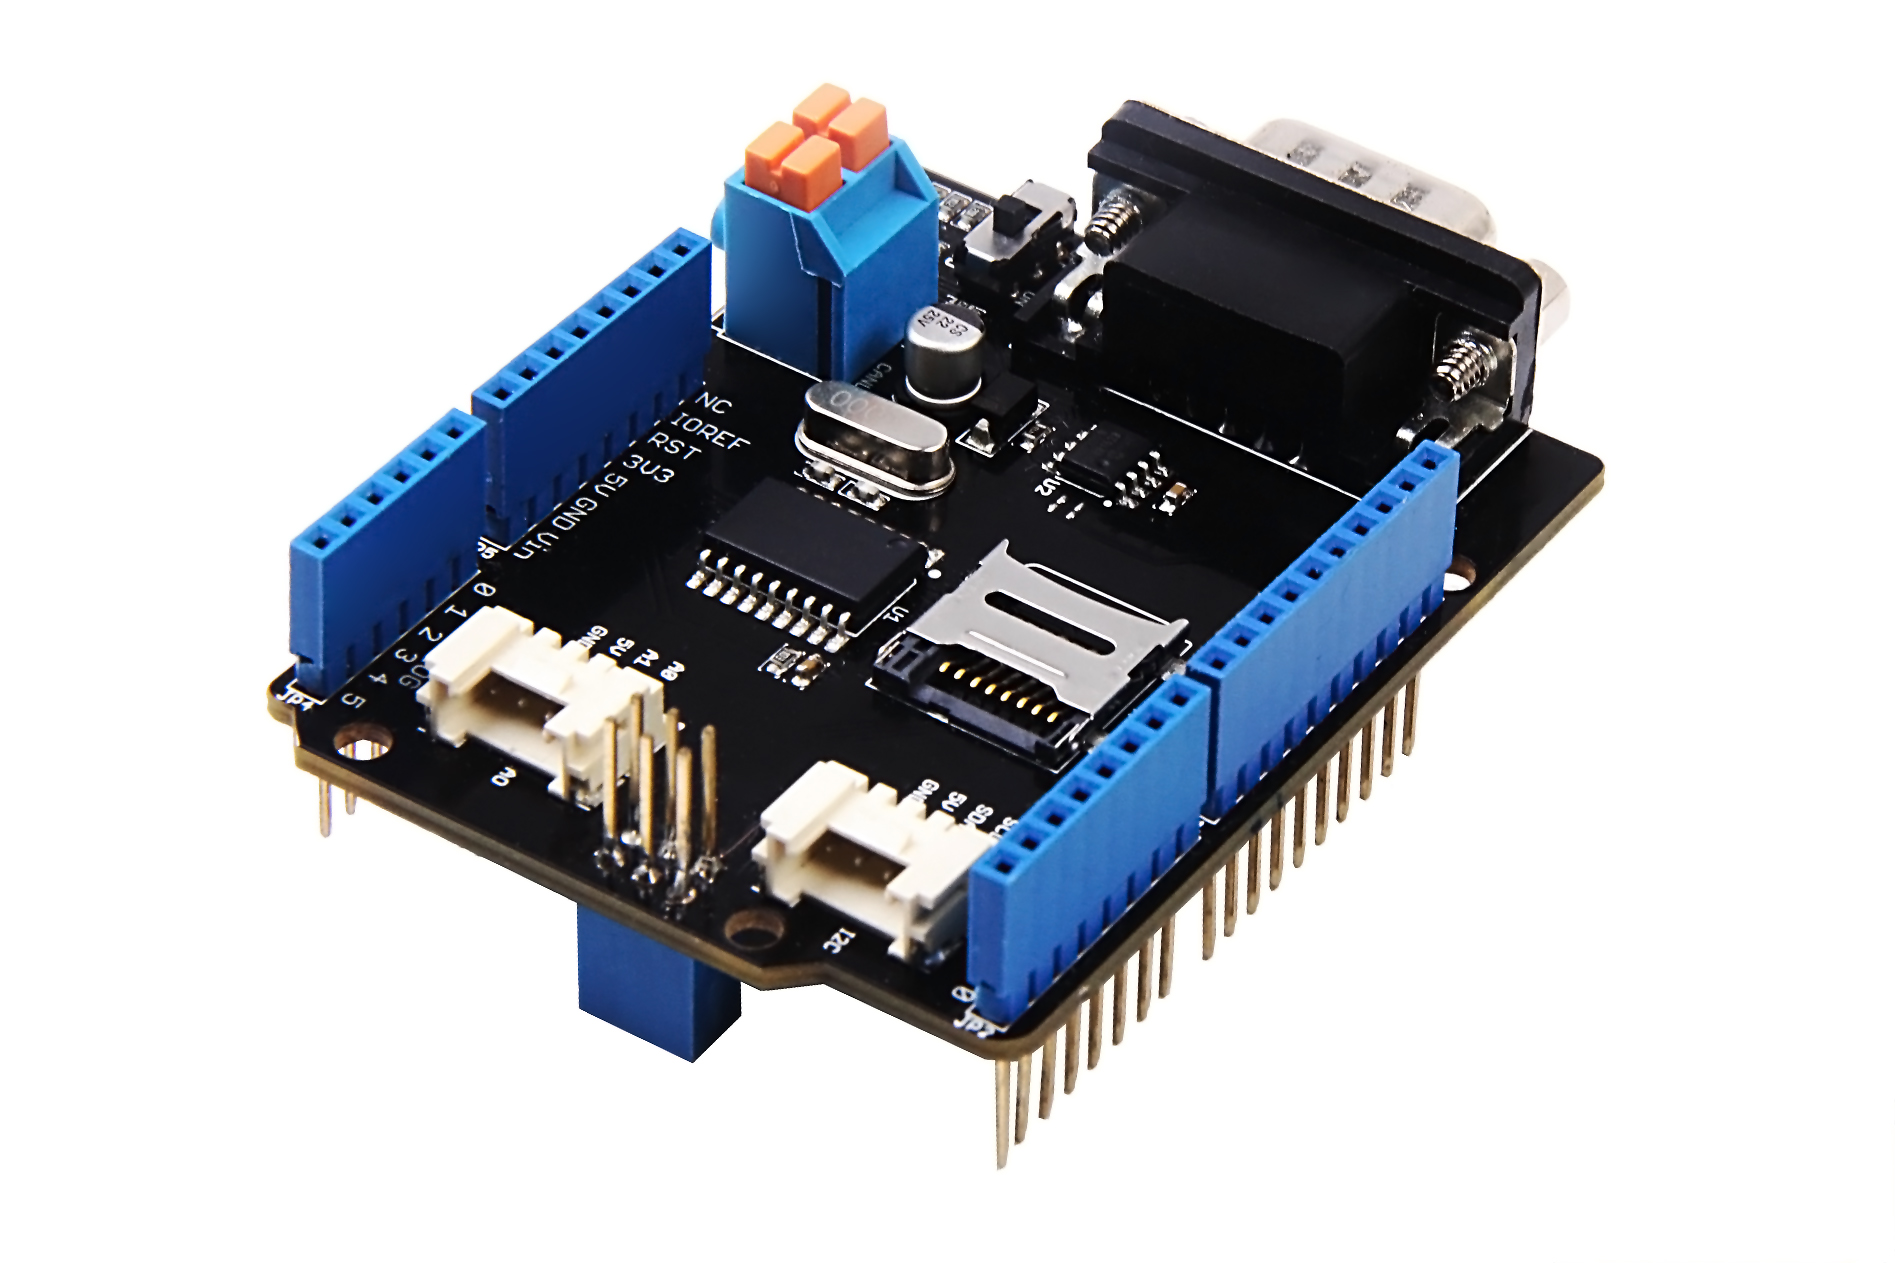
\includegraphics[height=1.2cm]{../../figures/r25_can_shield.jpg}\hspace{2mm}\parbox[b]{.6\linewidth}{\credit{CAN interface board for a microcontroller: Seeed Wiki, CC BY-SA 4.0, via Wikimedia Commons}}
\end{columns}
\vspace{1mm}
\gofurther{the CiA 402 drive profile defines one state machine and one set of objects (control word, status word, target position) so that every vendor's drive is commanded the same way over CANopen or EtherCAT.}
\end{frame}


% ---------------------------------------------------------------------
\begin{frame}{EtherCAT: processing on the fly}
\centering
\begin{tikzpicture}[font=\scriptsize]
  \begin{scope}
    \node[blk,fill=mkCream,draw=mkOrange] (m) at (0,0) {master};
    \foreach \i/\x in {1/2.6,2/5.0,3/7.4,4/9.8}{\node[blk] (s\i) at (\x,0) {drive \i};}
    \draw[sig,mkOrange] ($(m.east)+(0,.15)$) -- ($(s1.west)+(0,.15)$);
    \draw[sig,mkOrange] ($(s1.east)+(0,.15)$) -- ($(s2.west)+(0,.15)$);
    \draw[sig,mkOrange] ($(s2.east)+(0,.15)$) -- ($(s3.west)+(0,.15)$);
    \draw[sig,mkOrange] ($(s3.east)+(0,.15)$) -- ($(s4.west)+(0,.15)$);
    \draw[sig,mkMid] ($(s4.west)+(0,-.15)$) -- ($(s3.east)+(0,-.15)$);
    \draw[sig,mkMid] ($(s3.west)+(0,-.15)$) -- ($(s2.east)+(0,-.15)$);
    \draw[sig,mkMid] ($(s2.west)+(0,-.15)$) -- ($(s1.east)+(0,-.15)$);
    \draw[sig,mkMid] ($(s1.west)+(0,-.15)$) -- ($(m.east)+(0,-.15)$);
    \node[mkOrange] at (3.8,.5) {one frame passes all drives};
    \node[mkMid] at (3.8,-.55) {and comes back};
  \end{scope}
\end{tikzpicture}

\vspace{3mm}
\begin{columns}[T]
\column{.5\textwidth}
\begin{itemize}\small
\item Like a train passing stations: each drive \hl{unloads} its set-points and \hl{loads} its actual values while the frame rushes through (well under \SI{1}{\micro s} per drive).
\item A \term{working counter} in the frame tells the master that every drive answered.
\item \term{Distributed clocks}: all drives share one time base and act at the same instant.
\end{itemize}
\column{.47\textwidth}
\begin{keybox}[Example: 32 axes]
\small
1.\ $32\times\SI{12}{B}=\SI{384}{B}$ + \SI{52}{B} overhead\\
2.\ $\approx\SI{3500}{bit}$ at \SI{100}{Mbit/s} $\approx\SI{35}{\micro s}$\\
3.\ + delays $\approx\SI{30}{\micro s}$ $\Rightarrow$ fits a \SI{100}{\micro s} cycle
\end{keybox}
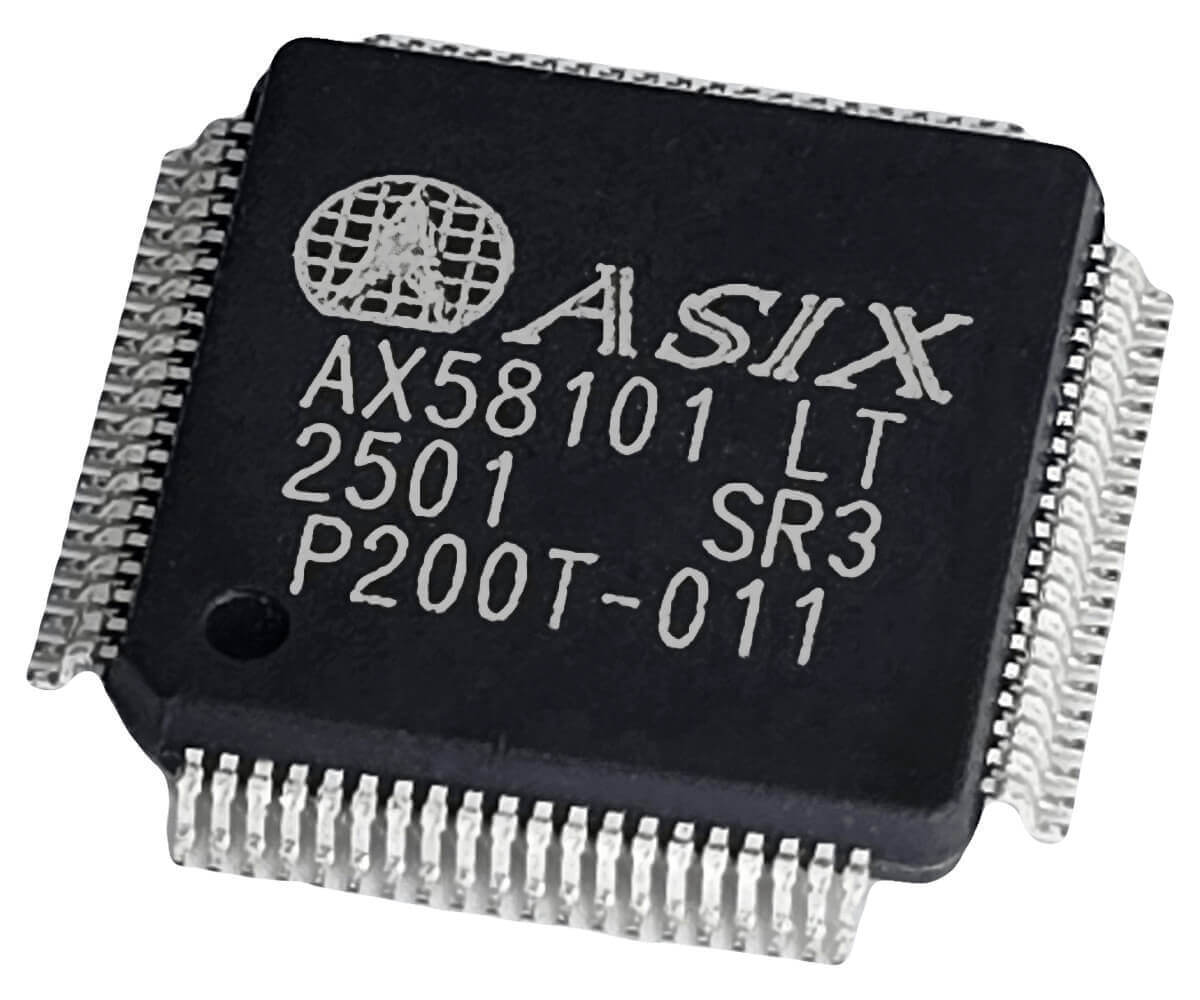
\includegraphics[height=1.0cm]{../../figures/d5_ethercat_esc.jpg}\\
\credit{EtherCAT slave controller IC: Allanchou1357, CC BY-SA 4.0, via Wikimedia Commons}
\end{columns}
\vspace{1mm}
\gofurther{distributed-clock details: propagation-delay measurement, drift compensation, SYNC0 events, sub-\si{\micro s} jitter.}
\end{frame}


% ---------------------------------------------------------------------
\begin{frame}{PROFINET, and comparing industrial networks}
\small
\renewcommand{\arraystretch}{1.15}
\begin{tabularx}{\linewidth}{@{}l l l X@{}}
\toprule
\textbf{Network} & \textbf{Speed} & \textbf{Typical cycle} & \textbf{Use in a robot cell}\\
\midrule
CAN / CANopen & \SI{1}{Mbit/s} & $\ge$\SI{1}{ms} & small robots, AMRs, grippers, sensors\\
EtherCAT & \SI{100}{Mbit/s} & \SI{62.5}{\micro s}--\SI{4}{ms} & robot joints, multi-axis motion\\
PROFINET RT & \SI{100}{Mbit/s} & \SIrange{1}{10}{ms} & PLC $\leftrightarrow$ I/O, robot, valves\\
PROFINET IRT & \SI{100}{Mbit/s} & \SI{31.25}{\micro s}--\SI{1}{ms} & synchronised motion\\
OPC UA & Ethernet & \SI{100}{ms}--s & cell data to HMI / MES / cloud\\
ROS 2 (DDS) & Ethernet & \SIrange{1}{100}{ms} & research, AMRs, vision and planning\\
\bottomrule
\end{tabularx}

\vspace{3mm}
\begin{columns}[T]
\column{.5\textwidth}
\begin{itemize}\small
\item \term{PROFINET}: Ethernet for PLCs; \term{RT} skips the slow TCP/IP layers, \term{IRT} reserves a fixed time slot in every cycle.
\item Like a motorway with a bus lane that is closed to all other traffic.
\end{itemize}
\column{.47\textwidth}
\begin{keybox}[How to choose]
\small By \hl{cycle time}, \hl{synchronisation}, number of devices and what the PLC / robot vendor supports --- not by bit rate alone.
\end{keybox}
\end{columns}
{\scriptsize\color{mkGray} Standards: ISO 11898 (CAN), IEC 61158 / 61784 (fieldbuses), IEC 62541 (OPC UA), IEC 61800-7 (drive profiles).}
\end{frame}

\begin{frame}{OPC UA: machines that describe themselves}
\begin{columns}[T]
\column{.5\textwidth}
\centering
\begin{tikzpicture}[font=\scriptsize,node distance=4mm]
  \node[blk,minimum width=2.4cm,fill=mkCream,draw=mkOrange] (srv) {OPC UA server\\in robot controller};
  \node[below=4mm of srv,draw=mkBlue,fill=white,thick,align=left,inner sep=3pt,font=\tiny] (tree) {%
    Robot\_1\\
    \ \ $\vdash$ State = \texttt{"Running"}\\
    \ \ $\vdash$ CycleTime = 8.4 s\\
    \ \ $\vdash$ Joint\_3/Temperature = 52 \textdegree C\\
    \ \ $\vdash$ Methods: Start(), Stop()};
  \node[blk,right=10mm of srv,fill=mkLight] (hmi) {HMI};
  \node[blk,below=4mm of hmi,fill=mkLight] (mes) {MES};
  \node[blk,below=4mm of mes,fill=mkLight] (cloud) {cloud\\dashboard};
  \foreach \c in {hmi,mes,cloud}{\draw[thick,mkMid,{Latex}-{Latex}] (srv.east) -- (\c.west);}
\end{tikzpicture}
\column{.47\textwidth}
\begin{itemize}\small
\item \term{OPC UA} = vendor-neutral way to exchange \emph{named, typed} data, not just raw bytes.
\item Each machine offers an \term{information model}: a tree of variables, methods and alarms with units.
\item Client--server (ask when needed) or publish--subscribe (broadcast changes).
\item Built-in security: certificates, encryption.
\item Not for fast control loops: typical \SI{100}{ms} or slower.
\end{itemize}
\gofurther{companion specifications (e.g.\ OPC UA for Robotics, VDMA 40010) define standard trees per machine type; OPC UA over TSN aims at real-time.}
\end{columns}
\end{frame}

\begin{frame}{ROS: the software glue of research and mobile robots}
\begin{columns}[T]
\column{.52\textwidth}
\centering
\begin{tikzpicture}[font=\scriptsize,
  nd/.style={draw=mkBlue,fill=mkPale,thick,ellipse,minimum width=1.7cm,minimum height=.7cm,align=center},
  tp/.style={draw=mkOrange,fill=mkCream,thick,rounded corners=1pt,font=\tiny\ttfamily,inner sep=2pt}]
  \node[nd] (cam) at (0,2.2) {camera\\driver};
  \node[nd] (det) at (3.2,2.2) {object\\detector};
  \node[nd] (lid) at (0,0) {LiDAR\\driver};
  \node[nd] (nav) at (3.2,0) {path\\planner};
  \node[nd] (base) at (3.2,-1.6) {motor\\controller};
  \node[tp] (t1) at (1.6,2.2) {/image};
  \node[tp] (t2) at (1.6,0) {/scan};
  \node[tp] (t3) at (3.2,1.1) {/objects};
  \node[tp] (t4) at (3.2,-.85) {/cmd\_vel};
  \draw[sig] (cam) -- (t1); \draw[sig] (t1) -- (det);
  \draw[sig] (lid) -- (t2); \draw[sig] (t2) -- (nav);
  \draw[sig] (det) -- (t3); \draw[sig] (t3) -- (nav);
  \draw[sig] (nav) -- (t4); \draw[sig] (t4) -- (base);
  \node[mkGray,align=left,anchor=west] at (-1,-1.6) {ellipse = node\\box = topic};
\end{tikzpicture}
\column{.45\textwidth}
\begin{itemize}\small
\item \term{ROS} (Robot Operating System) is not an OS but a \hl{middleware}: a set of libraries and tools.
\item Programs are \term{nodes}; they exchange messages on named \term{topics} (publish--subscribe), or call \term{services} and \term{actions}.
\item Like a radio: anyone may broadcast on a channel, anyone may listen.
\item ROS 2 uses DDS for transport; \texttt{ros2\_control} links to real hardware.
\end{itemize}
\begin{notebox}
\small Hard real-time loops (current, velocity) still run in the drive; ROS plans and coordinates.
\end{notebox}
\end{columns}
\end{frame}


% ---------------------------------------------------------------------
\begin{frame}{Synchronisation and latency: which loops may run over the bus?}
\centering
\begin{tikzpicture}[font=\scriptsize]
  \lbx{0}{1.2}{encoder}{mkSky!40}
  \lbx{1.2}{2.4}{wait\\for cycle}{mkPale}
  \lbx{2.4}{3.6}{bus to\\controller}{mkMid!25}
  \lbx{3.6}{5.4}{controller\\computes}{mkCream}
  \lbx{5.4}{6.6}{bus to\\drive}{mkMid!25}
  \lbx{6.6}{7.8}{apply}{mkPale}
  \lbx{7.8}{9.4}{current\\loop}{mkSky!40}
  \draw[{Latex}-{Latex},mkOrange,thick] (0,-.25) -- (9.4,-.25) node[midway,below]{total delay $T_d\approx 2$--$3$ bus cycles};
\end{tikzpicture}

\vspace{3mm}
\begin{columns}[T]
\column{.5\textwidth}
\begin{keybox}[Worked example]
\small
1.\ Bus cycle \SI{250}{\micro s}, $T_d=2.5\times250=\SI{625}{\micro s}$\\[1mm]
2.\ Position loop, $f_c=\SI{30}{Hz}$: $360\cdot30\cdot625\cdot10^{-6}=7^\circ$ \textcolor{mkGreen}{ok}\\[1mm]
3.\ Velocity loop, $f_c=\SI{200}{Hz}$: $45^\circ$ \textcolor{mkRed}{too much}
\end{keybox}
\column{.47\textwidth}
\begin{itemize}\small
\item Close the fast loops (current, velocity) \hl{inside the drive}.
\item Send only position set-points over the bus (CSP mode).
\item Shower analogy: a long pipe (delay) makes temperature control slow --- keep fast control close to the tap.
\item \term{Synchronisation}: all axes share one clock (EtherCAT distributed clocks, IEEE 1588 PTP), so a 6-axis path stays on track.
\end{itemize}
\end{columns}
\end{frame}


% ---------------------------------------------------------------------
\begin{frame}{Is the data valid? CRC, counters, watchdogs, timestamps}
\begin{columns}[T]
\column{.5\textwidth}
\begin{itemize}\small
\item \term{CRC}: detects bits damaged on the way. But a correct value can still be \emph{old}.
\item \term{Counters}: a number that increases every cycle; a frozen counter = lost data.
\item \term{Watchdog}: a timer that trips if no fresh data arrives in time.
\item \term{Timestamp}: age of a value $=t_\text{now}-t_\text{sample}$.
\item \term{Plausibility}: is the value possible? e.g.\ $i_a+i_b+i_c=0$.
\end{itemize}
\column{.47\textwidth}
\centering
\begin{tikzpicture}[font=\scriptsize,node distance=4mm]
  \node[blk,minimum width=4.4cm] (rx) {packet received};
  \node[blk,below=of rx,minimum width=4.4cm] (crc) {CRC ok?};
  \node[blk,below=of crc,minimum width=4.4cm] (seq) {counter advanced, fresh?};
  \node[blk,below=of seq,minimum width=4.4cm] (pl) {value plausible?};
  \node[blk,below=of pl,minimum width=4.4cm,fill=mkCream,draw=mkGreen] (use) {use value, reset watchdog};
  \draw[sig] (rx) -- (crc); \draw[sig] (crc) -- (seq); \draw[sig] (seq) -- (pl); \draw[sig] (pl) -- (use);
  \node[blk,right=5mm of seq,fill=mkRed!15,draw=mkRed,minimum width=1.4cm] (err) {stop safely,\\alarm};
  \draw[sig,mkRed] (crc.east) -| (err.north);
  \draw[sig,mkRed] (seq) -- (err);
  \draw[sig,mkRed] (pl.east) -| (err.south);
\end{tikzpicture}
\end{columns}
\end{frame}


% ---------------------------------------------------------------------
\begin{frame}{Check your understanding: communication}
\begin{keybox}[Check your understanding]
\large
\begin{enumerate}
\item Which network would you choose (a) between robot joints, (b) between the cell and the factory MES? Why?
\item A bus has a total delay of \SI{1}{ms}. How much phase does this cost a loop with $f_c=\SI{100}{Hz}$? Would you close that loop over the bus?
\item A value arrives with a correct CRC but is five cycles old. Which mechanism catches this?
\end{enumerate}
\end{keybox}
\end{frame}


% ---------------------------------------------------------------------
\begin{frame}{Summary and key terms: communication and integration}
\begin{columns}[T]
\column{.52\textwidth}
\begin{itemize}\small
\item Packets = header + data + CRC; buses exchange them every cycle.
\item CAN/CANopen: robust, priority arbitration, $\ge$\SI{1}{ms} cycles.
\item PROFINET RT/IRT for PLC cells; OPC UA for named data to MES; ROS 2 to glue robot software.
\item EtherCAT: one frame through all drives, \SI{100}{\micro s} cycles, common clock.
\item Delay costs phase: close fast loops inside the drive; check freshness of data.
\end{itemize}
\column{.45\textwidth}
\begin{defbox}[Key terms]
\small
\term{packet} header + data + check\\
\term{fieldbus} machine network with fixed timing\\
\term{OPC UA} self-describing machine data\\
\term{ROS topic} named publish--subscribe channel\\
\term{latency} age of data on arrival\\
\term{watchdog} timer that trips on missing data
\end{defbox}
{\scriptsize\color{mkGray} ETG.1000 / IEC 61158; IEC 62541; ISO 11898; [Quigley et al., 2009]; [Macenski et al., 2022].}
\end{columns}
\end{frame}


% =====================================================================
\section{6.8 System-integration case study and course wrap-up}

\begin{frame}{Case study: a vision-guided conveyor-picking cell}
\centering
\begin{tikzpicture}[font=\scriptsize]
  % conveyor
  \draw[thick,mkGray,fill=mkLight] (0,0) rectangle (8.5,.4);
  \foreach \x in {.2,8.3}{\draw[mkGray,thick] (\x,.2) circle (.2);}
  \draw[-{Latex},mkGray,thick] (3.3,-.25) -- (5.0,-.25) node[right]{$v=\SI{0.5}{m/s}$};
  \foreach \x/\r in {1.0/25,2.6/-30,5.8/50}{\draw[fill=mkOrange!60,draw=mkOrange,rotate around={\r:(\x,.6)}] (\x-.25,.45) rectangle (\x+.25,.75);}
  % encoder
  \fill[mkSky] (.2,.2) circle (.09); \node[below] at (.2,-.05) {encoder};
  % camera + light
  \draw[fill=mkNavy] (2.3,2.4) rectangle (2.9,2.8); \node[above] at (2.6,2.8) {camera};
  \draw[mkSky,dashed] (2.45,2.4) -- (1.6,.45); \draw[mkSky,dashed] (2.75,2.4) -- (3.6,.45);
  % photo-eye
  \draw[mkRed,thick] (1.5,.45) -- (1.5,1.3); \fill[mkRed] (1.5,1.35) circle (.06); \node[left,mkRed] at (1.5,1.2) {photo-eye};
  % robot
  \fill[mkNavy] (6.5,.95) rectangle (7.1,1.1);
  \draw[very thick,mkBlue] (6.8,1.1) -- (6.8,2.3) -- (6.0,2.6) -- (5.8,1.3);
  \draw[mkNavy,thick] (5.65,1.3) -- (5.95,1.3); \node[right] at (6.9,1.9) {robot + vacuum gripper};
  % light curtain
  \draw[mkRed,dashed,thick] (8.9,0) -- (8.9,2.8); \node[mkRed,align=center] at (8.9,3.05) {light curtain};
  % network
  \node[blk,fill=mkCream,draw=mkOrange] (plc) at (10.8,2.3) {safety PLC\\+ cell PLC};
  \node[blk] (rc) at (10.8,1.0) {robot\\controller};
  \node[blk,fill=mkLight] (mes) at (10.8,-.3) {MES\\(OPC UA)};
  \draw[thick,mkMid] (plc) -- (rc) node[midway,right,font=\tiny]{PROFINET};
  \draw[thick,mkGray] (rc) -- (mes);
\end{tikzpicture}

\vspace{2mm}
\begin{columns}[T]
\column{.5\textwidth}
\begin{itemize}\small
\item Parts arrive randomly placed; the robot must pick 60 per minute.
\item Today's topics meet: vision (6.4), sampling of the encoder (6.5), filtering (6.6), networks (6.7).
\end{itemize}
\column{.47\textwidth}
\begin{itemize}\small
\item Plus last week: kinematics (W2D1--2), safety (W2D4), servo loops (W1D5).
\item Question: \hl{will the gripper hit the part?}
\end{itemize}
\end{columns}
\end{frame}

% ---------------------------------------------------------------------
\begin{frame}{Case study: who talks to whom, and how fast}
\begin{columns}[T]
\column{.55\textwidth}
\centering
\begin{tikzpicture}[font=\scriptsize,node distance=5mm]
  \node[blk,fill=mkSky!40] (pe) {photo-eye};
  \node[blk,right=of pe] (cam) {camera};
  \node[blk,right=of cam] (vis) {vision PC};
  \node[blk,below=8mm of cam,fill=mkSky!40] (enc) {conveyor\\encoder};
  \node[blk,right=of enc,fill=mkCream,draw=mkOrange] (rc) {robot\\controller};
  \node[blk,right=of rc] (dr) {6 joint\\drives};
  \draw[sig,mkRed] (pe) -- (cam) node[midway,above,font=\tiny]{trigger};
  \draw[sig] (cam) -- (vis) node[midway,above,font=\tiny]{GigE};
  \draw[sig] (vis) -- (rc) node[midway,right,font=\tiny]{Ethernet};
  \draw[sig] (enc) -- (rc) node[midway,below,font=\tiny]{latched count};
  \draw[sig] (rc) -- (dr) node[midway,below,font=\tiny]{EtherCAT};
  \draw[sig,mkRed,dashed] (pe.south) |- ($(enc.west)+(0,.15)$);
  \node[mkRed,font=\tiny,align=right,anchor=north east] at ($(pe.south)+(-0.05,-.15)$) {same trigger\\latches count};
\end{tikzpicture}
\column{.43\textwidth}
\small
\renewcommand{\arraystretch}{1.12}
\begin{tabularx}{\linewidth}{@{}X r@{}}
\toprule
\textbf{Step} & \textbf{Time}\\
\midrule
trigger + exposure & \SI{2}{ms}\\
image transfer & \SI{15}{ms}\\
image processing & \SI{60}{ms}\\
send result & \SI{3}{ms}\\
\midrule
total vision latency & \SI{80}{ms}\\
\bottomrule
\end{tabularx}
\end{columns}

\vspace{3mm}
\begin{notebox}
\small In \SI{80}{ms} the part travels $0.5\cdot0.080=\SI{40}{mm}$ --- far more than the gripper tolerance of $\pm\SI{2}{mm}$. The answer is not a faster PC but a \hl{time stamp}: latch the encoder count at the moment of exposure.
\end{notebox}
\end{frame}

% ---------------------------------------------------------------------
\begin{frame}{Case study: conveyor tracking, step by step}
\begin{columns}[T]
\column{.5\textwidth}
\begin{eqbox}
\vspace{-2mm}
\[ x_\text{part}(t)=x_\text{image}+\Delta n\cdot s_\text{enc} \]
\vspace{-4mm}
\end{eqbox}
{\small $x_\text{image}$: position from vision at exposure; $\Delta n$: encoder counts since exposure; $s_\text{enc}$: belt travel per count [mm].}

\vspace{2mm}
\begin{itemize}\small
\item The robot controller follows the moving part frame like a \term{user frame} on wheels (W2D3).
\item The encoder is sampled every robot cycle; its resolution and timing set the error.
\end{itemize}
\column{.47\textwidth}
\begin{keybox}[Worked example]
\small
1.\ Roll diameter \SI{100}{mm}: circumference $\pi\cdot100=\SI{314}{mm}$\\[1mm]
2.\ Encoder 1000 counts/rev $\Rightarrow s_\text{enc}=\SI{0.314}{mm}$\\[1mm]
3.\ Vision: part at $x_\text{image}=\SI{120}{mm}$; since exposure $\Delta n=1900$ counts\\[1mm]
4.\ $x_\text{part}=120+1900\cdot0.314=\SI{717}{mm}$ $\rightarrow$ robot target
\end{keybox}
\end{columns}
\end{frame}

% ---------------------------------------------------------------------
\begin{frame}{Case study: the error budget}
\begin{columns}[T]
\column{.52\textwidth}
\small
\renewcommand{\arraystretch}{1.12}
\begin{tabularx}{\linewidth}{@{}X r@{}}
\toprule
\textbf{Error source} & \textbf{$\pm$ mm}\\
\midrule
vision: 1 px at \SI{0.5}{mm/px} & 0.50\\
hand--eye calibration & 0.50\\
encoder: 1 count & 0.31\\
timing jitter \SI{1}{ms} at \SI{0.5}{m/s} & 0.50\\
robot repeatability & 0.05\\
\midrule
worst case (sum) & 1.86\\
statistical (root of sum of squares) & \hl{0.92}\\
\bottomrule
\end{tabularx}
\column{.45\textwidth}
\begin{eqbox}
\vspace{-2mm}
\[ e_\text{RSS}=\sqrt{e_1^2+e_2^2+\dots+e_n^2} \]
\vspace{-4mm}
\end{eqbox}
\begin{itemize}\small
\item Independent errors rarely all peak together: RSS is the realistic estimate.
\item Both stay below the gripper tolerance of $\pm\SI{2}{mm}$: \textcolor{mkGreen}{\textbf{the design works}}.
\item Biggest terms first: better lens or lighting, careful calibration, hardware time stamps.
\end{itemize}
\end{columns}
\end{frame}

% ---------------------------------------------------------------------
\begin{frame}{Case study: commissioning the cell}
\begin{columns}[T]
\column{.5\textwidth}
\centering
\begin{tikzpicture}[font=\scriptsize,node distance=2.5mm,
  st/.style={draw=mkBlue,fill=mkPale,thick,rounded corners=2pt,minimum width=5.4cm,minimum height=6mm,align=left,text width=5.2cm}]
  \node[st] (a) {\textbf{1} Wiring and I/O check, network diagnostics};
  \node[st,below=of a] (b) {\textbf{2} Safety functions validated (light curtain, E-stop, PL)};
  \node[st,below=of b] (c) {\textbf{3} Drive tuning and robot frames (base, tool, user)};
  \node[st,below=of c] (d) {\textbf{4} Camera and hand--eye calibration};
  \node[st,below=of d] (e) {\textbf{5} Conveyor tracking test at low speed};
  \node[st,below=of e,fill=mkCream,draw=mkOrange] (f) {\textbf{6} Full-speed run, cycle time and error log};
  \foreach \u/\v in {a/b,b/c,c/d,d/e,e/f}{\draw[sig] (\u) -- (\v);}
\end{tikzpicture}
\column{.47\textwidth}
\begin{itemize}\small
\item \term{System integration}: making separately good parts work as \hl{one} system.
\item Inside-out order: each step relies on the one before (like tuning loops inner to outer, W1D5).
\item \term{FAT} (factory acceptance test) at the integrator, \term{SAT} (site acceptance test) at the customer.
\item Log data with time stamps: most integration bugs are timing bugs.
\end{itemize}
\end{columns}
\end{frame}

% ---------------------------------------------------------------------
\begin{frame}{Check your understanding: integration case study}
\begin{keybox}[Check your understanding]
\large
\begin{enumerate}
\item The conveyor speed doubles to \SI{1}{m/s}. Which entry of the error budget changes, and what is the new RSS value?
\item Why does latching the encoder count at the camera trigger make the vision delay harmless?
\item Why are safety functions validated \emph{before} the robot runs at full speed?
\end{enumerate}
\end{keybox}
\end{frame}

% ---------------------------------------------------------------------
\begin{frame}{Course wrap-up: ten days, one robot}
\centering
\begin{tikzpicture}[font=\scriptsize,node distance=1.6mm,
  day/.style={draw=mkBlue,fill=mkPale,thick,rounded corners=2pt,minimum height=6mm,align=left,text width=6.3cm}]
  \node[day] (d1) {\textbf{W1D1} Motors: DC, BLDC, PMSM, stepper; electrical + mechanical models};
  \node[day,below=of d1] (d2) {\textbf{W1D2} Gearboxes, linear actuators, motor sizing; modelling, Laplace};
  \node[day,below=of d2] (d3) {\textbf{W1D3} Block diagrams, Bode plots, PID, stability margins};
  \node[day,below=of d3] (d4) {\textbf{W1D4} Filters, digital control, manipulator control; drives, PWM};
  \node[day,below=of d4] (d5) {\textbf{W1D5} FOC, cascaded loops, tuning, trajectories + feedforward};
  \node[day,right=4mm of d1,fill=mkCream,draw=mkOrange] (e1) {\textbf{W2D1} Resonance; robot anatomy; transforms; forward kinematics};
  \node[day,below=of e1,fill=mkCream,draw=mkOrange] (e2) {\textbf{W2D2} Inverse kinematics, Jacobian, dynamics, path planning; automation};
  \node[day,below=of e2,fill=mkCream,draw=mkOrange] (e3) {\textbf{W2D3} Robot applications, work cells, PLCs, robot programming};
  \node[day,below=of e3,fill=mkCream,draw=mkOrange] (e4) {\textbf{W2D4} Material handling, safety standards; sensors I};
  \node[day,below=of e4,fill=mkCream,draw=mkOrange] (e5) {\textbf{W2D5} Vision, sampling, filters, networks, integration};
\end{tikzpicture}

\vspace{3mm}
\begin{columns}[T]
\column{.48\textwidth}
\centering\small \textcolor{mkBlue}{\textbf{Week 1: make one joint move well}}\\
{\footnotesize actuators $\rightarrow$ control $\rightarrow$ servo drives}
\column{.48\textwidth}
\centering\small \textcolor{mkOrange}{\textbf{Week 2: make many joints do useful work}}\\
{\footnotesize mechanisms $\rightarrow$ manufacturing $\rightarrow$ sensors \& integration}
\end{columns}
\end{frame}

% ---------------------------------------------------------------------
\begin{frame}{Course wrap-up: every topic in one robot joint}
\centering
\begin{tikzpicture}[font=\scriptsize]
  \node[blk,fill=mkLight] (plc) at (0,2.2) {PLC / cell\\program};
  \node[blk] (traj) at (2.4,2.2) {trajectory +\\IK};
  \node[blk] (pos) at (4.8,2.2) {position\\loop};
  \node[blk] (vel) at (7.0,2.2) {velocity\\loop};
  \node[blk] (cur) at (9.2,2.2) {current\\(FOC) + PWM};
  \node[blk,fill=mkCream,draw=mkOrange] (mot) at (11.6,2.2) {motor +\\gearbox};
  \node[blk,fill=mkCream,draw=mkOrange] (arm) at (11.6,0) {link + payload};
  \node[blk,fill=mkSky!40] (sen) at (7.0,0) {encoder, F/T,\\camera};
  \node[blk] (flt) at (4.8,0) {ADC +\\filters};
  \node[blk,fill=mkLight] (net) at (1.2,0) {network\\EtherCAT / OPC UA};
  \draw[sig] (plc) -- (traj); \draw[sig] (traj) -- (pos); \draw[sig] (pos) -- (vel); \draw[sig] (vel) -- (cur); \draw[sig] (cur) -- (mot);
  \draw[sig] (mot) -- (arm); \draw[sig] (arm) -- (sen); \draw[sig] (sen) -- (flt);
  \draw[sig] (flt) -- (pos); \draw[sig] (flt.north east) -- (vel.south west); \draw[sig] (net) -- (plc); \draw[sig,dashed] (flt) -- (net);
  \foreach \n/\t/\p in {plc/{5.4, 5.5}/above,traj/{4.4, 4.7}/above,pos/{2.5, 3.4}/above,vel/{3.4, 3.5}/above,cur/{3.2, 3.3}/above,mot/{1.2--1.7}/above,
    arm/{4.6, 3.7}/below,sen/{6.1--6.4}/below,flt/{6.5, 6.6}/below,net/{6.7}/below}{
    \node[\p=1mm of \n,font=\tiny\bfseries,text=mkOrange] {\t};}
\end{tikzpicture}

\vspace{4mm}
\begin{keybox}[The course in one sentence]
\small A robot is good when its \hl{mechanics}, \hl{actuators}, \hl{control loops}, \hl{sensors} and \hl{networks} are designed together --- the weakest link sets the performance.
\end{keybox}
{\scriptsize\color{mkGray} Orange numbers: curriculum session codes where each block was taught.}
\end{frame}

% ---------------------------------------------------------------------
\begin{frame}{Course wrap-up: ten principles to take home}
\begin{columns}[T]
\column{.5\textwidth}
\begin{enumerate}\small
\item Size the actuator for the \emph{whole} motion: RMS torque, peak, heat (W1D2).
\item Model first, then measure and compare (W1D2--3).
\item Feedback needs margins: delay and filters eat phase (W1D3--4).
\item Inner loops 3--10$\times$ faster than outer loops (W1D5).
\item Feedforward does the work, feedback fixes the errors (W1D5).
\end{enumerate}
\column{.48\textwidth}
\begin{enumerate}\small
\setcounter{enumi}{5}
\item Kinematics links joints and the tool: watch singularities (W2D1--2).
\item Design the cell around cycle time, reach and tooling (W2D3).
\item Safety is designed in from day one, not added (W2D4).
\item A measurement is only as good as its sensor, sampling and filter (W2D4--5).
\item Synchronise and time-stamp everything (W2D5).
\end{enumerate}
\end{columns}
\end{frame}

% ---------------------------------------------------------------------
\begin{frame}{Day summary}
\begin{columns}[T]
\column{.52\textwidth}
\begin{itemize}\small
\item \textbf{6.4} Camera model, calibration, pose, stereo, hand--eye.
\item \textbf{6.5} Nyquist, aliasing, quantisation, ADC types, delay.
\item \textbf{6.6} Low-pass, moving average, FIR/IIR, notch, filtered derivative, fusion.
\item \textbf{6.7} CAN, EtherCAT, PROFINET, OPC UA, ROS; latency and synchronisation.
\item \textbf{6.8} Conveyor-tracking cell: time stamps and an error budget.
\end{itemize}
\column{.45\textwidth}
\begin{defbox}[Key terms of the day]
\small
\term{intrinsics}, \term{hand--eye calibration}, \term{disparity},
\term{Nyquist frequency}, \term{aliasing}, \term{quantisation},
\term{IIR / FIR}, \term{notch}, \term{complementary filter}, \term{Kalman gain},
\term{fieldbus}, \term{OPC UA}, \term{ROS topic}, \term{latency},
\term{time stamp}, \term{error budget}
\end{defbox}
\end{columns}
\end{frame}

% ---------------------------------------------------------------------
\begin{frame}{Course wrap-up: where to go next}
\begin{columns}[T]
\column{.5\textwidth}
\begin{itemize}\small
\item \textbf{Control}: state-space design, observers, robust and optimal control.
\item \textbf{Robotics}: dynamics and force control, motion planning, mobile robots and SLAM.
\item \textbf{Vision and AI}: 3D perception, learning-based grasping.
\item \textbf{Practice}: build a small robot arm or AMR with ROS 2; program a PLC; tune a real servo.
\end{itemize}
\column{.47\textwidth}
\begin{keybox}[Thank you]
\small Questions and discussion. Next time you see a robot cell, try to spot its \hl{actuators}, its \hl{sensors}, its \hl{loops} and its \hl{networks} --- you now know how each of them works.
\end{keybox}
\vspace{2mm}
\centering
\IfFileExists{../../figures/d4_kuka_robot.jpg}{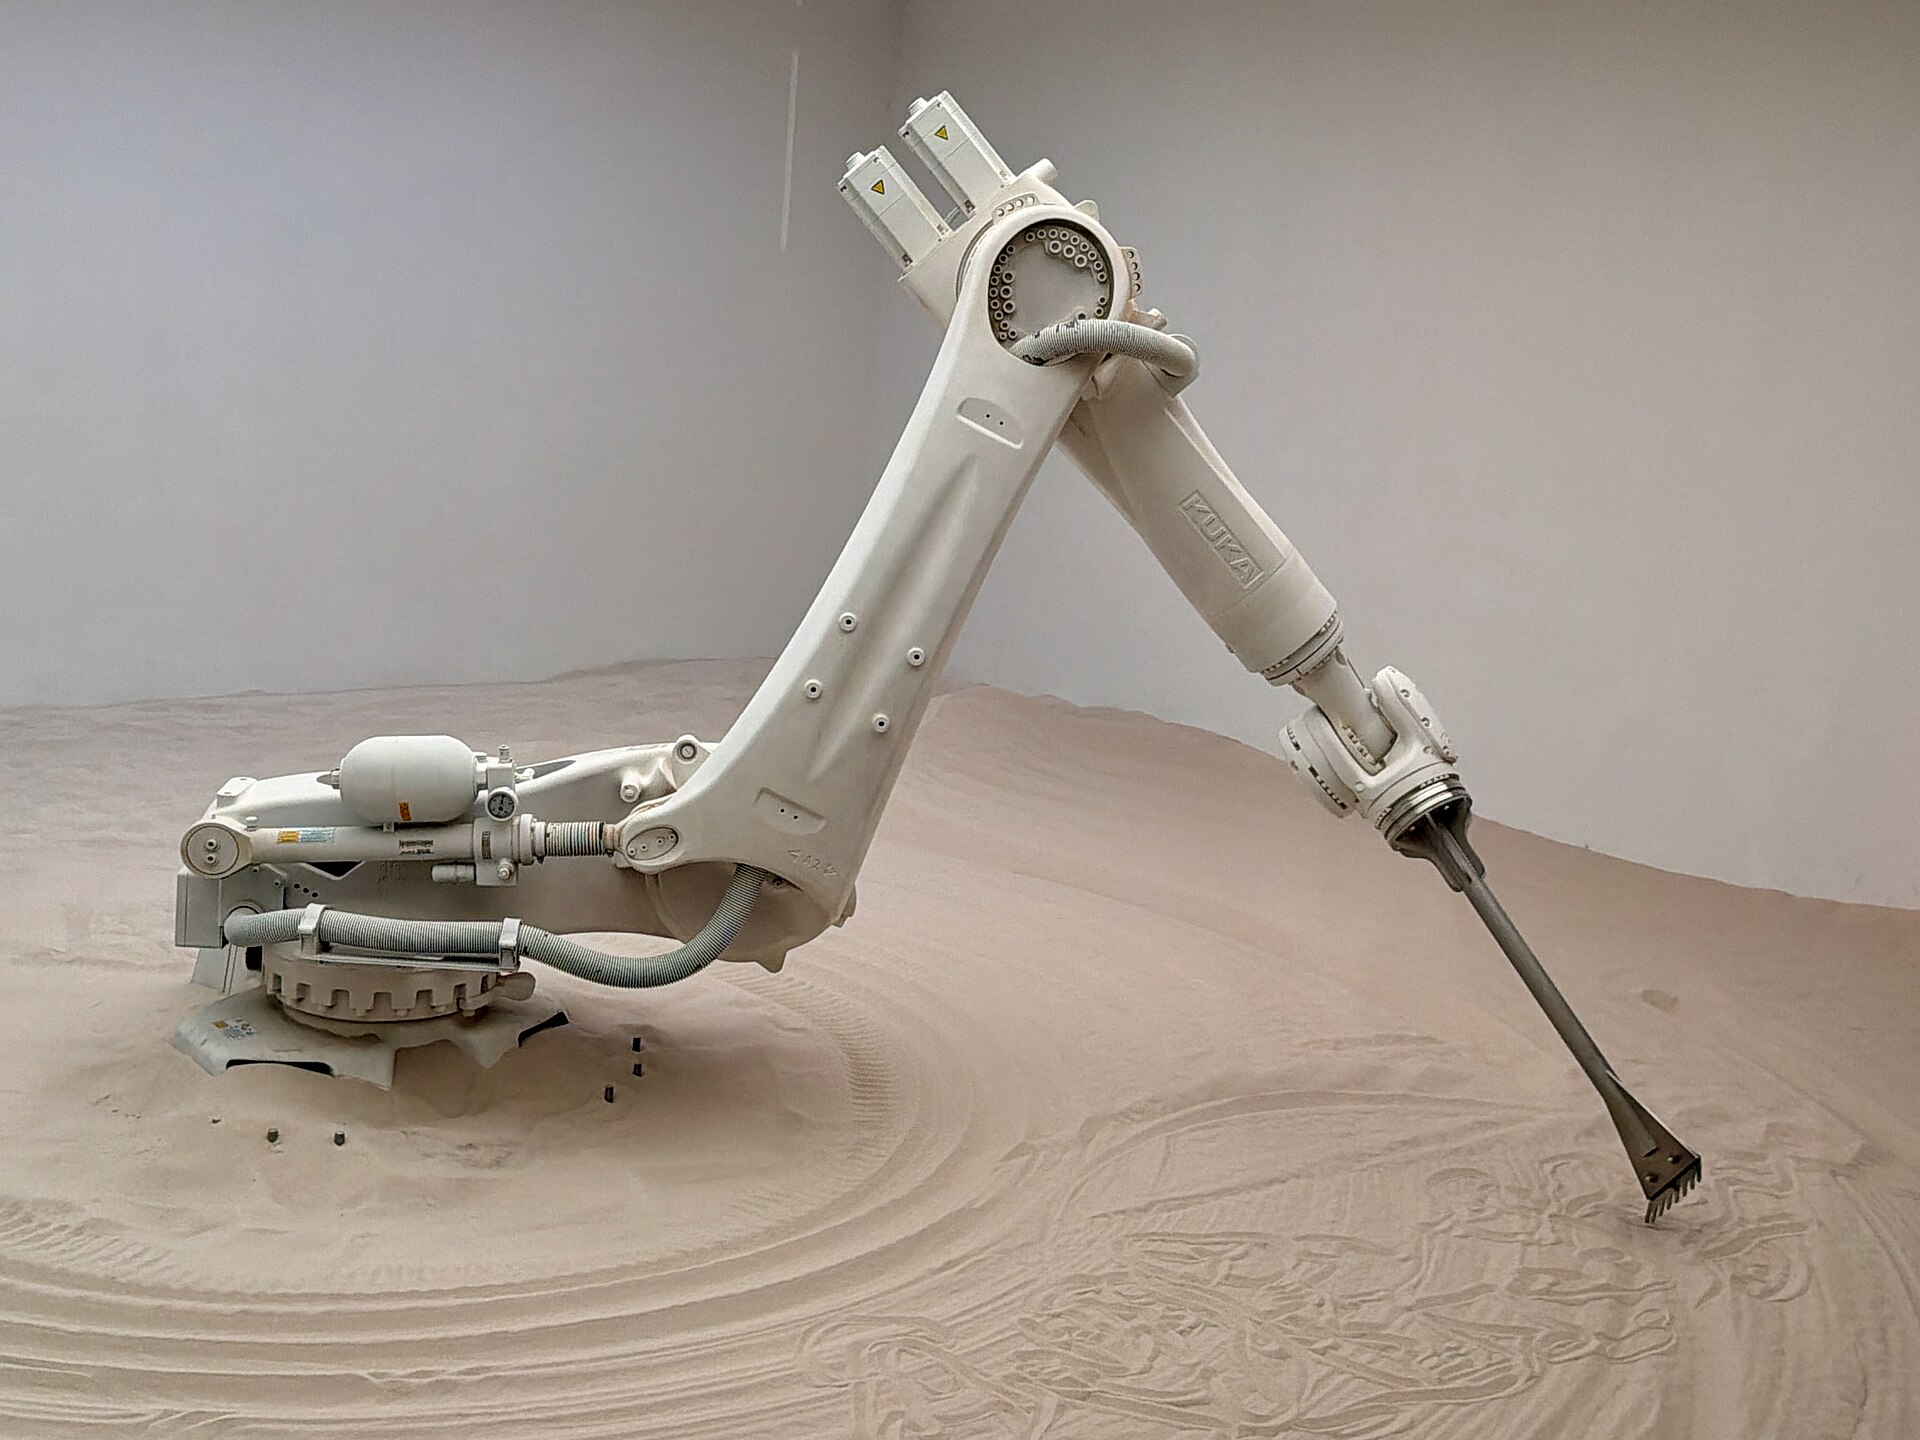
\includegraphics[height=2.3cm]{../../figures/d4_kuka_robot.jpg}\\
\credit{\KukaCredit}}{}
\end{columns}
\end{frame}

% ---------------------------------------------------------------------
\begin{frame}{Figure credits}
\scriptsize
All plots and diagrams not listed here are original drawings made for this course (TikZ / pgfplots; data generated by \texttt{w2d5/data/gen\_data.py} and \texttt{day5/data/gen\_data.py}).

\vspace{2mm}
\renewcommand{\arraystretch}{1.15}
\begin{tabularx}{\linewidth}{@{}l X l l@{}}
\toprule
\textbf{File} & \textbf{Wikimedia Commons title} & \textbf{Author} & \textbf{License}\\
\midrule
\texttt{r25\_vision\_camera.jpg} & SVS Vistek EXO Tracer 8318.jpg & Ginkgomaier & CC BY-SA 4.0\\
\texttt{r25\_checkerboard.png} & Chessboard calibration setup.png & Brian moore81 & CC BY-SA 4.0\\
\texttt{r25\_realsense.jpg} & Intel Realsense depth camera D435.jpg & Marc Auledas & CC BY-SA 4.0\\
\texttt{r25\_mv\_system.jpg} & Machine Vision System.jpg & European Editors & CC BY-SA 4.0\\
\texttt{r25\_can\_shield.jpg} & CAN BUS Shield V2.jpg & Seeed Wiki & CC BY-SA 4.0\\
\texttt{d4\_kuka\_robot.jpg} & KUKA industrial robotic arm performing ``The Beach'' by Roy Nachum - 02.jpg & Oleg Yunakov & CC BY-SA 4.0\\
\texttt{d5\_ethercat\_esc.jpg} & ASIX AX58101 EtherCAT SubDevice Controller.jpg & Allanchou1357 & CC BY-SA 4.0\\
\bottomrule
\end{tabularx}

\vspace{1mm}
All via Wikimedia Commons (commons.wikimedia.org); licences as stated.
\end{frame}

% ---------------------------------------------------------------------
\begin{frame}{References}
\scriptsize
\begin{itemize}
\item P.~Corke, \emph{Robotics, Vision and Control}, 2nd ed., Springer, 2017.
\item R.~Szeliski, \emph{Computer Vision: Algorithms and Applications}, 2nd ed., Springer, 2022.
\item Z.~Zhang, ``A flexible new technique for camera calibration'', \emph{IEEE Trans.\ PAMI} 22(11), 2000.
\item R.~Y.~Tsai, R.~K.~Lenz, ``A new technique for fully autonomous and efficient 3D robotics hand/eye calibration'', \emph{IEEE Trans.\ Robotics and Automation} 5(3), 1989.
\item A.~V.~Oppenheim, R.~W.~Schafer, \emph{Discrete-Time Signal Processing}, 3rd ed., Pearson, 2010.
\item G.~F.~Franklin, J.~D.~Powell, M.~L.~Workman, \emph{Digital Control of Dynamic Systems}, 3rd ed., Addison-Wesley, 1998.
\item J.~Fraden, \emph{Handbook of Modern Sensors}, 5th ed., Springer, 2016.
\item B.~Siciliano, O.~Khatib (eds.), \emph{Springer Handbook of Robotics}, 2nd ed., Springer, 2016.
\item S.~Thrun, W.~Burgard, D.~Fox, \emph{Probabilistic Robotics}, MIT Press, 2005.
\item M.~Quigley et al., ``ROS: an open-source Robot Operating System'', ICRA Workshop on Open Source Software, 2009; S.~Macenski et al., ``Robot Operating System 2'', \emph{Science Robotics} 7(66), 2022.
\item ISO 11898 (CAN); IEC 61158 / IEC 61784 (fieldbuses, EtherCAT, PROFINET); IEC 62541 (OPC UA); IEC 61800-7 (drive profiles); IEEE 1588 (PTP); ISO 10218 (robot safety).
\end{itemize}
\end{frame}

\end{document}

